% Created 2023-06-08 Thu 11:31
% Intended LaTeX compiler: pdflatex
\documentclass[10pt,table,dvipsnames,compress]{beamer}
\usepackage[utf8]{inputenc}
\usepackage[T1]{fontenc}
\usepackage{graphicx}
\usepackage{longtable}
\usepackage{wrapfig}
\usepackage{rotating}
\usepackage[normalem]{ulem}
\usepackage{amsmath}
\usepackage{amssymb}
\usepackage{capt-of}
\usepackage{hyperref}
\usetheme{default}
\useinnertheme{rounded}
\useoutertheme[subsection=false]{miniframes}
\date{}
\title{forestatrisk: a Python package for modelling and forecasting deforestation}
\title[forestatrisk]{forestatrisk: a Python package for modelling and forecasting deforestation}
\usepackage{lmodern}
\usepackage{pgf}
\usepackage{color}
\usepackage[english,french]{babel}
\definecolor{vertmoyen}{RGB}{51,110,23} % vert moyen
\definecolor{blueFRB}{HTML}{31859c}
\usecolortheme[named=blueFRB]{structure}
\usepackage{tabularx} % varier la largeur du tableau
\usepackage{layout}
\setlength{\LTleft}{-5cm plus 1 fill}
\setlength{\LTright}{-5cm plus 1 fill}
\usepackage{booktabs}
\usepackage{arydshln} %% dashlines for tabular
\newcommand{\logit}{\text{logit}}
\newcommand{\bs}[1]{\boldsymbol{#1}}
\newcommand{\R}{\textnormal{\sffamily\bfseries R}}
\newcommand{\pkg}[1]{{\fontseries{b}\selectfont #1}}
\newcolumntype{C}[1]{>{\centering\arraybackslash}m{#1}}

\setbeamertemplate{footline}[frame number]
\setbeamertemplate{frametitle}{%
\usebeamerfont{frametitle}\insertframetitle%
\vphantom{g} % To avoid fluctuations per frame
\par
\centering 
\includegraphics[width=\textwidth]{figs/Barre_couleur}
}
\beamertemplatenavigationsymbolsempty

% Logo
\newif\ifplacelogo % create a new conditional
\logo{\ifplacelogo
\includegraphics[width=0.6\textwidth]{figs/partners_logos}\fi}

%Call table of contents at the beginning of each section
\AtBeginSection[]{
\placelogotrue
\begin{frame}
\frametitle{Plan}
\begin{columns}[c]
\begin{column}{0.5\textwidth}
\tableofcontents[sections=1,currentsection]
\vspace{0.5cm}
\tableofcontents[sections=2,currentsection]
\end{column}
\begin{column}{0.5\textwidth}
\tableofcontents[sections=3,currentsection]
\vspace{0.5cm}
\tableofcontents[sections=4,currentsection]
\end{column}
\end{columns}
\end{frame}
\placelogofalse
}

\AtBeginSubsection[]{}

\hypersetup{
colorlinks=true,
linkcolor=Black,
filecolor=Maroon,
citecolor=Blue,
urlcolor=Maroon}

% Disable monospaced font for URLs
\urlstyle{same}

\hypersetup{
 pdfauthor={Ghislain Vieilledent},
 pdftitle={forestatrisk: a Python package for modelling and forecasting deforestation},
 pdfkeywords={},
 pdfsubject={},
 pdfcreator={Emacs 28.2 (Org mode 9.6.4)}, 
 pdflang={English}}
\begin{document}


% {
%   % Use background image
%   \usebackgroundtemplate{%
%     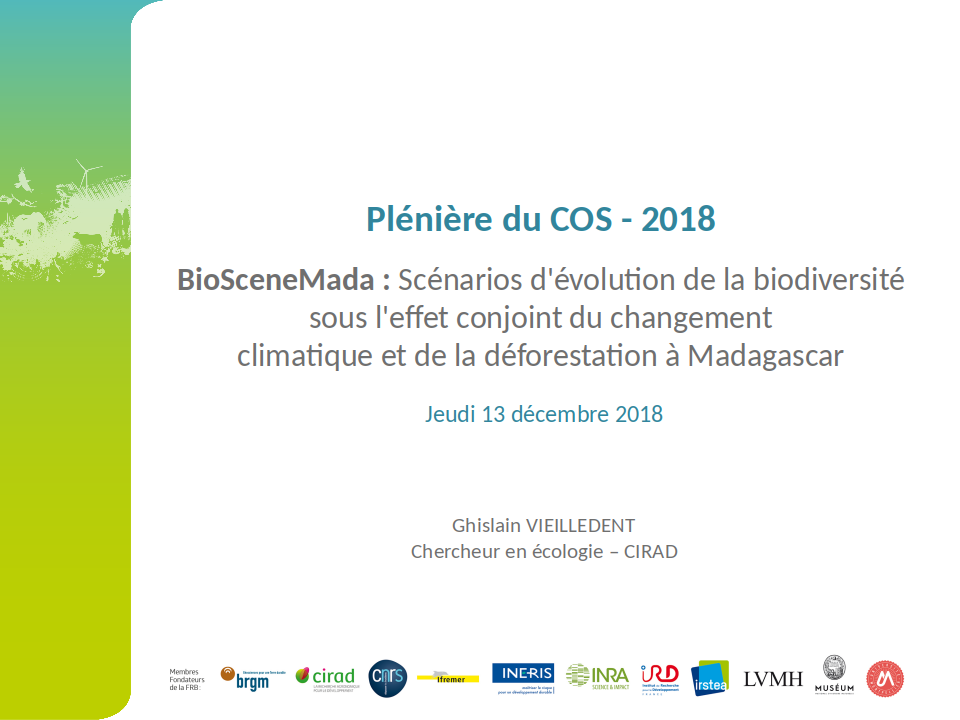
\includegraphics[height=\paperheight,width=\paperwidth]{figs/Masque.png}
%   }
%   \setbeamertemplate{navigation symbols}{}
%   % Remove shadow from block
%   \setbeamertemplate{blocks}[rounded][shadow=false]
%   \begin{frame}[plain]
%   \end{frame}
% }

% Title page
{
  \setbeamertemplate{navigation symbols}{}
  \begin{frame}[plain, noframenumbering]
  \begin{center}
  \small{\textbf{Meeting with EFI and COCOBOD -- June 08, 2023}}
  \end{center}
  \vspace{-0.5cm}
  \titlepage % Presentation first page
  \vspace{-3cm}
  \begin{center}
    
\includegraphics[width=\textwidth]{figs/Barre_couleur}
    
    \vspace{0.25cm}
    
    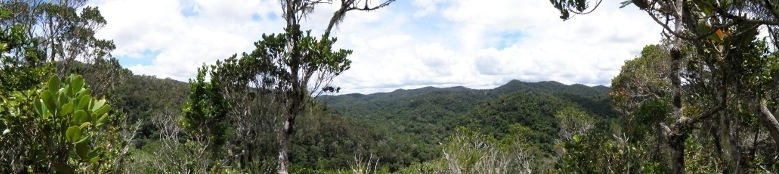
\includegraphics[width=10cm]{figs/Banniere}
    
    \small{Ghislain VIEILLEDENT$^{1, 2}$\hspace{0.25cm}Christelle VANCUTSEM$^{2}$\hspace{0.25cm}Frédéric ACHARD$^{2}$}
      
    \vspace{0.25cm}
    
    {\scriptsize
      \begin{tabular}{l}
        $[1]$ \textbf{Cirad} UMR AMAP, $[2]$ \textbf{EC JRC} Forests and bioeconomy unit
      \end{tabular}
    }
    
    
\includegraphics[width=0.8\textwidth]{figs/partners_logos}
    
  \end{center}
  \end{frame}
}

% %%%%%%%%%%%%%%%%%%%%%%%%%%%%%%%%%%%%%%%%%%%%%%%%%%%%%%%%%%%%%%%%

\placelogotrue
\begin{frame}
  \frametitle{Plan}
  \begin{columns}[c]
    \begin{column}{0.5\textwidth}
      \tableofcontents[sections=1]
      \vspace{0.5cm}
      \tableofcontents[sections=2]
    \end{column}
    \begin{column}{0.5\textwidth}
        \tableofcontents[sections=3]
        \vspace{0.5cm}
        \tableofcontents[sections=4]
    \end{column}
  \end{columns}
\end{frame}
\placelogofalse

\section{Introduction}
\label{sec:org20ea72a}
\subsection{Context}
\label{sec:org252f1c3}
\begin{frame}[label={sec:orgd788218}]{Context}
\begin{block}{Risk mapping}
\begin{itemize}
\item Need for estimating the spatial risk of deforestation in the tropics.
\item At high resolution, on large spatial scale.
\end{itemize}
\end{block}

\begin{block}{Usage}
\begin{itemize}
\item Conservation planning (hotspots of deforestation).
\item Jurisdictional REDD+:
\begin{itemize}
\item Allocating deforestation.
\item Building reference scenario of deforestation and carbon emissions.
\end{itemize}
\end{itemize}
\end{block}
\end{frame}

\begin{frame}[label={sec:org750b790}]{State-of-the-art}
\begin{itemize}
\item Existing software: Dinamica-EGO, Land Change Modeller, and CLUE.
\item Limitations:
\begin{itemize}
\item Might not be open source, cross-platform, scriptable, and user-friendly.
\item Do not account for the spatial autocorrelation of the residuals.
\item Algorithms (genetic algorithms, artificial neural networks, or machine learning algorithms) having the tendency to overfit the data.
\item Applications to large spatial scales (e.g., at the country or continental scale) with high resolution data (e.g., \(\leq\) 30 m) has not yet been demonstrated.
\end{itemize}
\end{itemize}
\end{frame}

\subsection{Software}
\label{sec:org414a46e}
\begin{frame}[label={sec:org930252f},fragile]{Software}
 \begin{itemize}
\item \texttt{forestatrisk} Python package.
\item Process large rasters by blocks (no memory issues).
\item Several statistical models: iCAR, GLM, RF, etc.
\item Set of functions for sampling, modelling, forecasting, validating.
\end{itemize}

\begin{center}
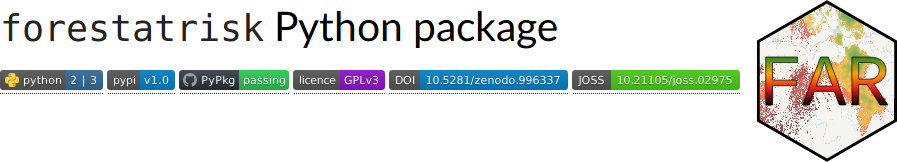
\includegraphics[width=0.8\textwidth]{figs/far-Python}\\
Article: \textbf{Vieilledent} 2021, \emph{JOSS}, doi: \href{https://doi.org/10.21105/joss.02975}{10.21105/joss.02975}\\
Website: \url{https://ecology.ghislainv.fr/forestatrisk}
\end{center}
\end{frame}

\section{Methods}
\label{sec:orgbc3e2a5}
\subsection{Data}
\label{sec:orgd024f4b}

\begin{frame}[label={sec:org9f549d7}]{Historical deforestation maps}
\begin{itemize}
\item We need an historical deforestation map.
\item At least between two dates.
\item Possible sources:
\begin{itemize}
\item Global Forest Change (GFC).
\item Tropical Moist Forest (TMF).
\item Map provided by National Authorities.
\end{itemize}
\end{itemize}

\vspace{0.25cm}
\centering 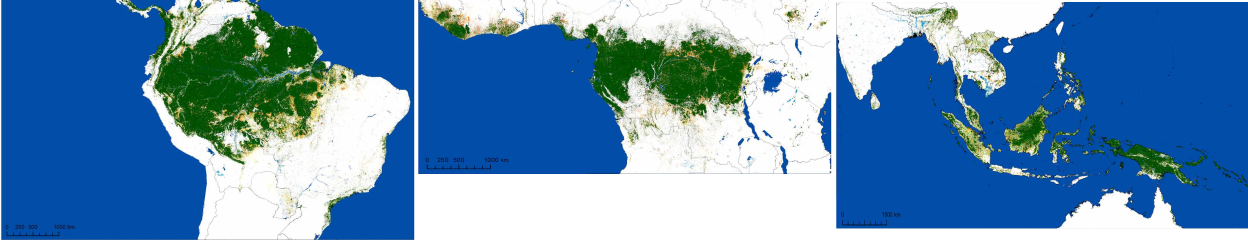
\includegraphics[width=\textwidth]{figs/Vancutsem2021-maps-wide}
\end{frame}

\begin{frame}[label={sec:org90c4f1a}]{Example for DRC}
\begin{columns}
\begin{column}{0.5\columnwidth}
\begin{itemize}
\item Example for DRC
\item Using the Tropical Moist Forest (TMF) dataset.
\item Three dates: 2000--2010--2020.
\item Makes it possible to account for the distance to past deforestation.
\end{itemize}
\end{column}

\begin{column}{0.5\columnwidth}
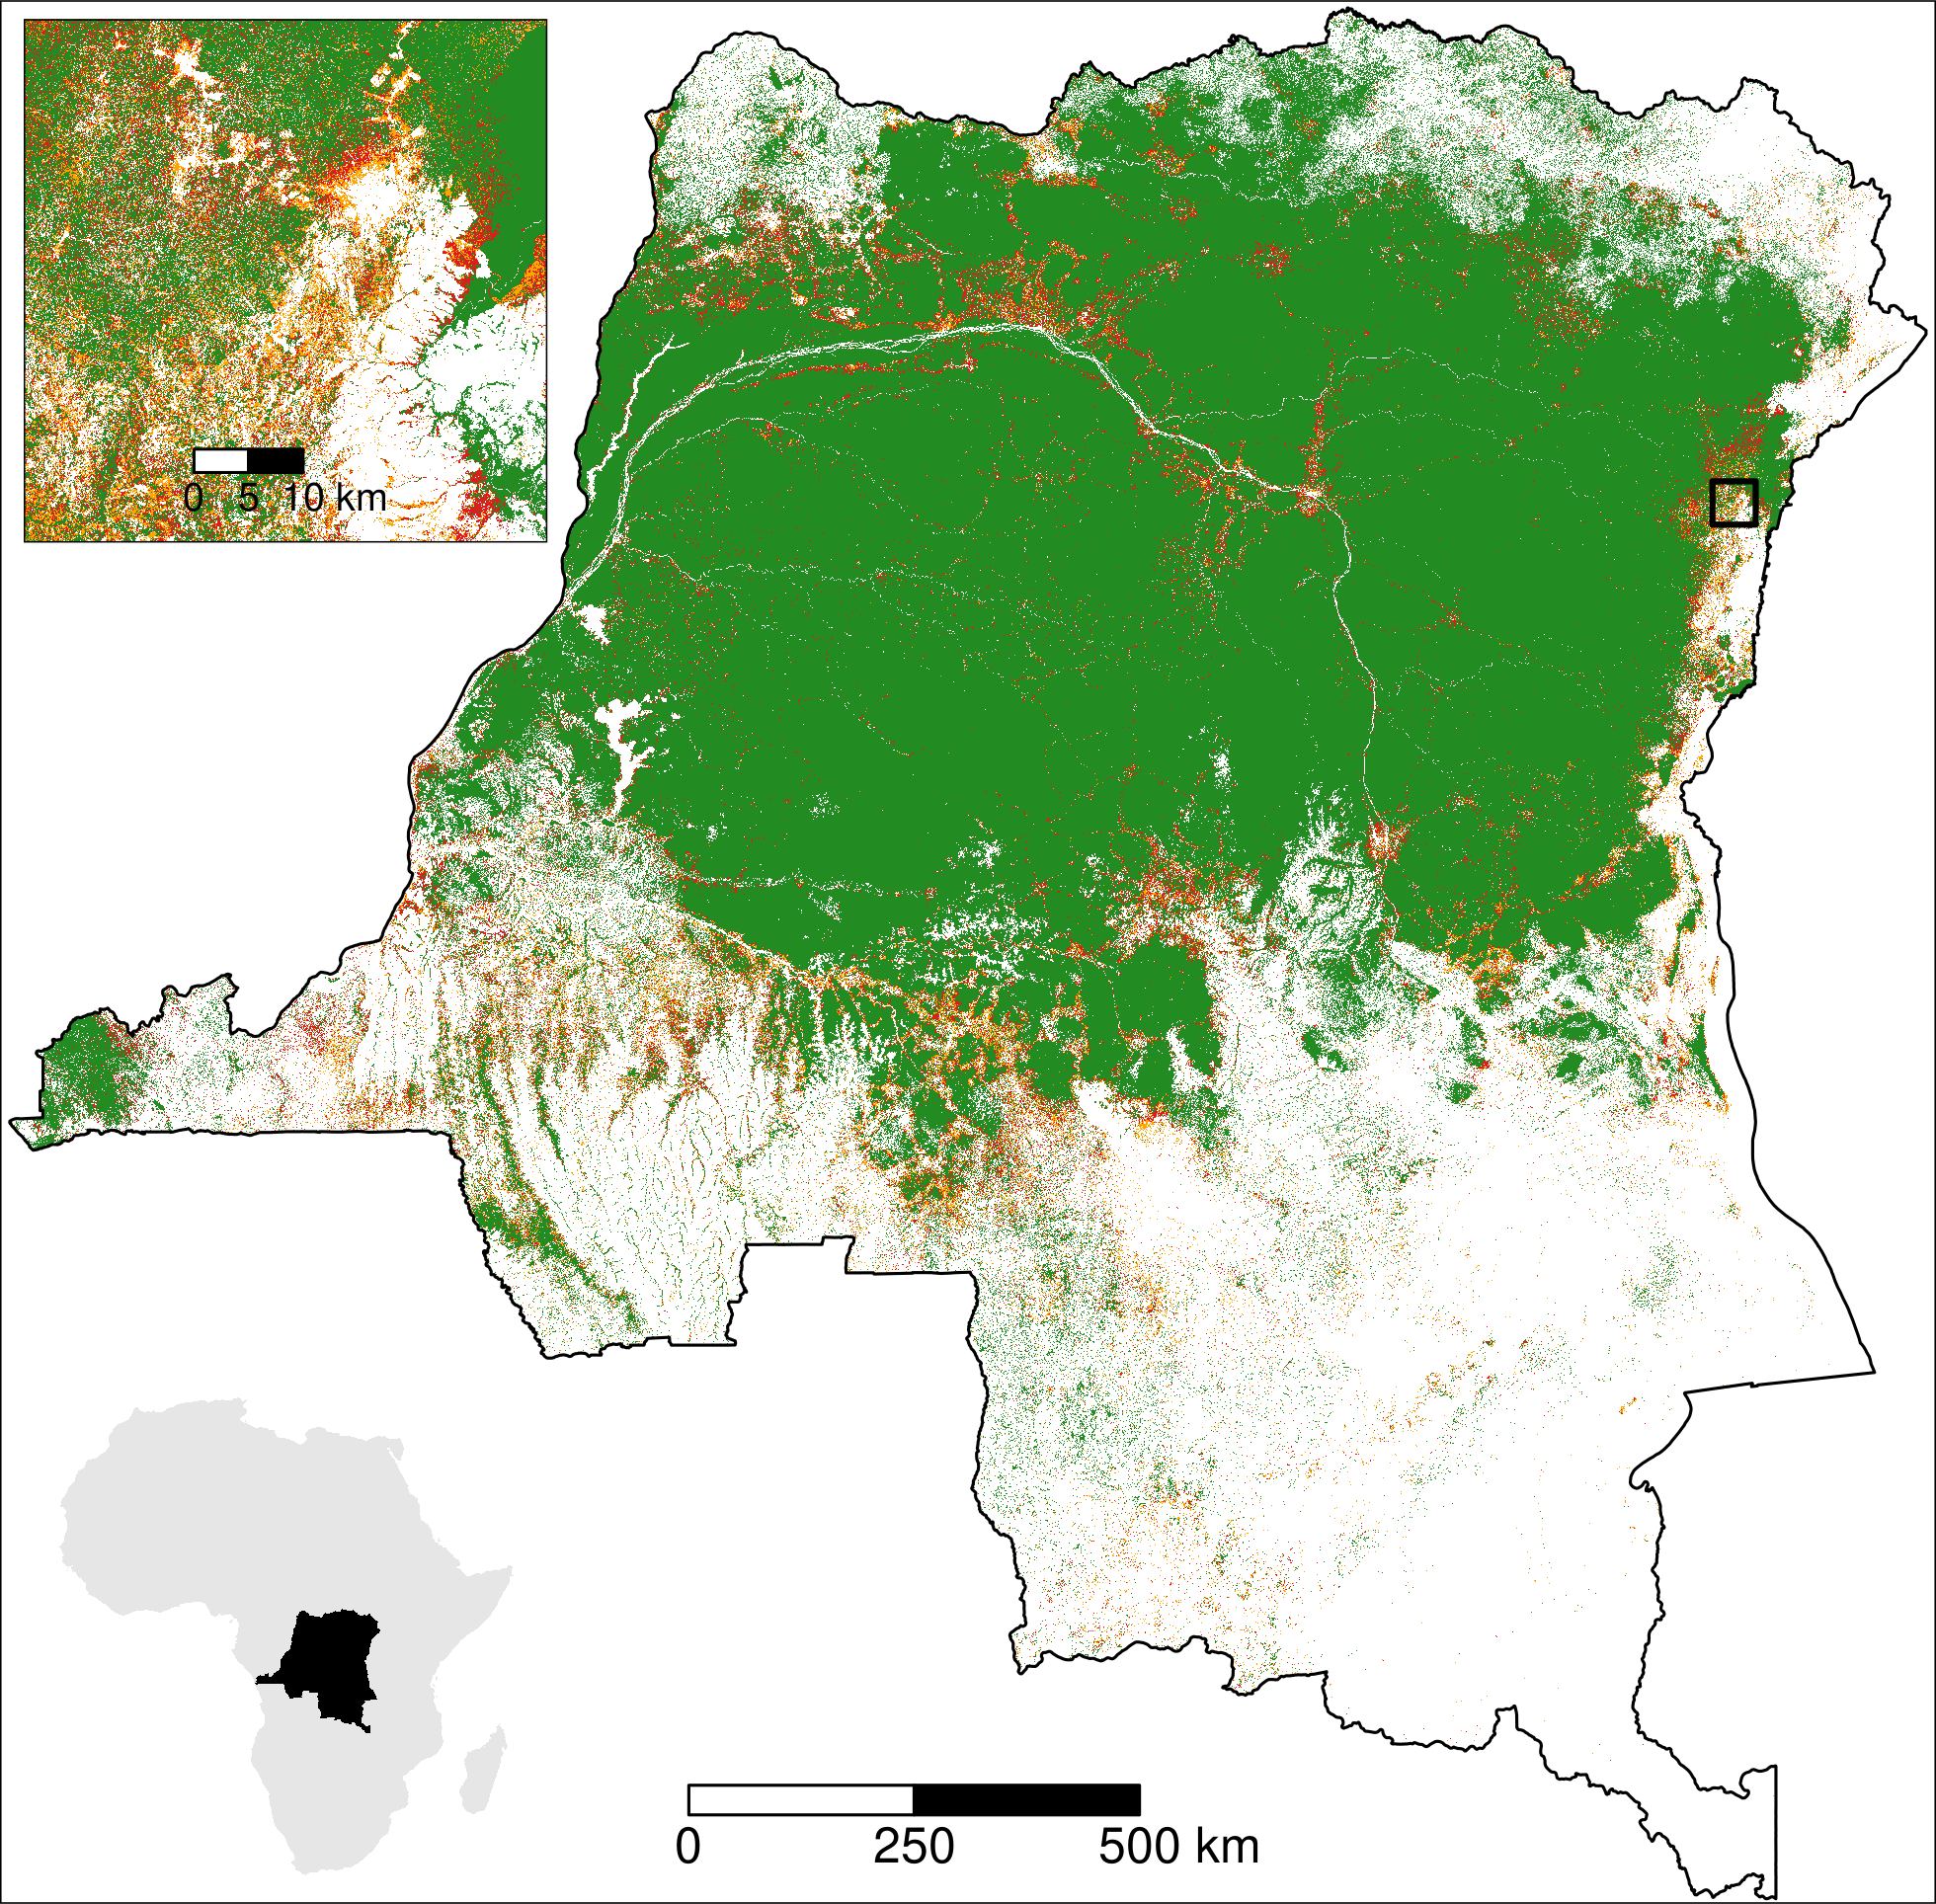
\includegraphics[width=\textwidth]{figs/sm/fcc123}

\structure{Past deforestation 2000--2010--2020 in DRC}
\end{column}
\end{columns}
\end{frame}

\begin{frame}[label={sec:org99fd0be}]{TMF dataset}
\centering 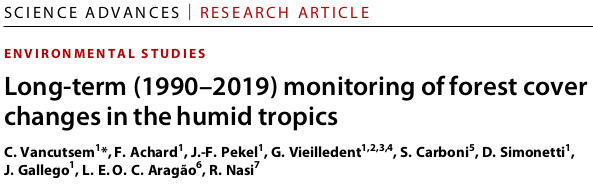
\includegraphics[width=8cm]{figs/Vancutsem2021}

\structure{Vancutsem et al.} 2021, \emph{Science Advances}, doi:\href{https//doi.org10.1126/sciadv.abe1603}{10.1126/sciadv.abe1603}

\begin{itemize}
\item Tropical Moist Forest (TMF)
\item 1990--2022: Annual deforestation, degradation, regeneration
\end{itemize}
\end{frame}

\begin{frame}[label={sec:org968ebfa}]{TMF dataset}
\begin{itemize}
\item Full Landsat archive (1982--2022), 30m pixel, time-series analysis.
\item Classification tree based on expert knowledge.
\item Tropical deforestation was underestimated (-33\% in 2000--2012, Hansen
et al. 2013).
\item Maps and data: \url{https://forobs.jrc.ec.europa.eu/TMF/}.
\end{itemize}

\vspace{0.25cm}
\centering 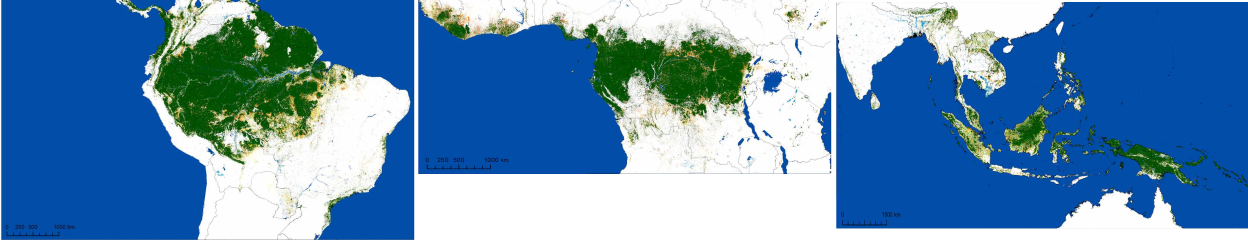
\includegraphics[width=\textwidth]{figs/Vancutsem2021-maps-wide}
\end{frame}

\begin{frame}[label={sec:orgba7ed77}]{TMF dataset}
\begin{itemize}
\item Precise enough to visually identify the causes of deforestation
(logging, fires, agriculture)
\end{itemize}

\centering 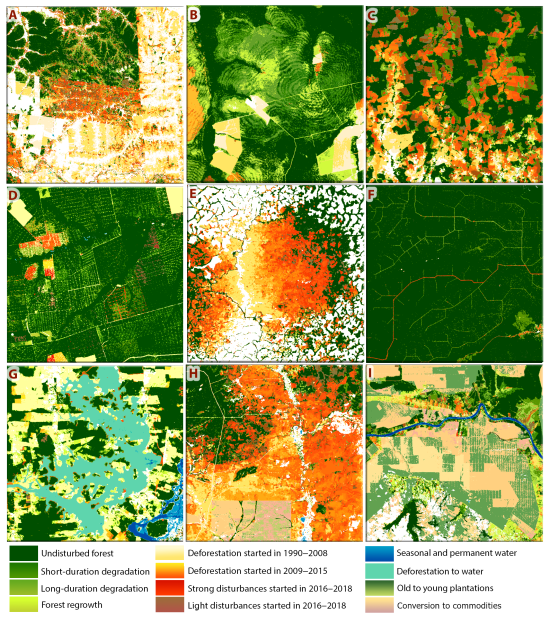
\includegraphics[height=0.7\textheight]{figs/Vancutsem2021-patterns}
\end{frame}


\begin{frame}[label={sec:orgf8378d5}]{Spatial variables}
\begin{itemize}
\item Height explanatory variables
\end{itemize}

\centering 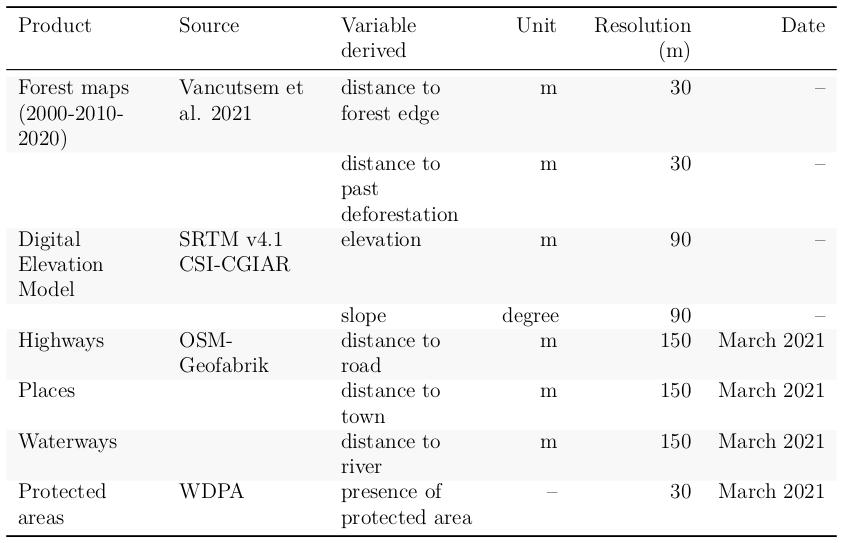
\includegraphics[width=0.7\textwidth]{figs/variables-tab}
\end{frame}

\begin{frame}[label={sec:org4ddf9e6}]{Spatial variables}
\centering 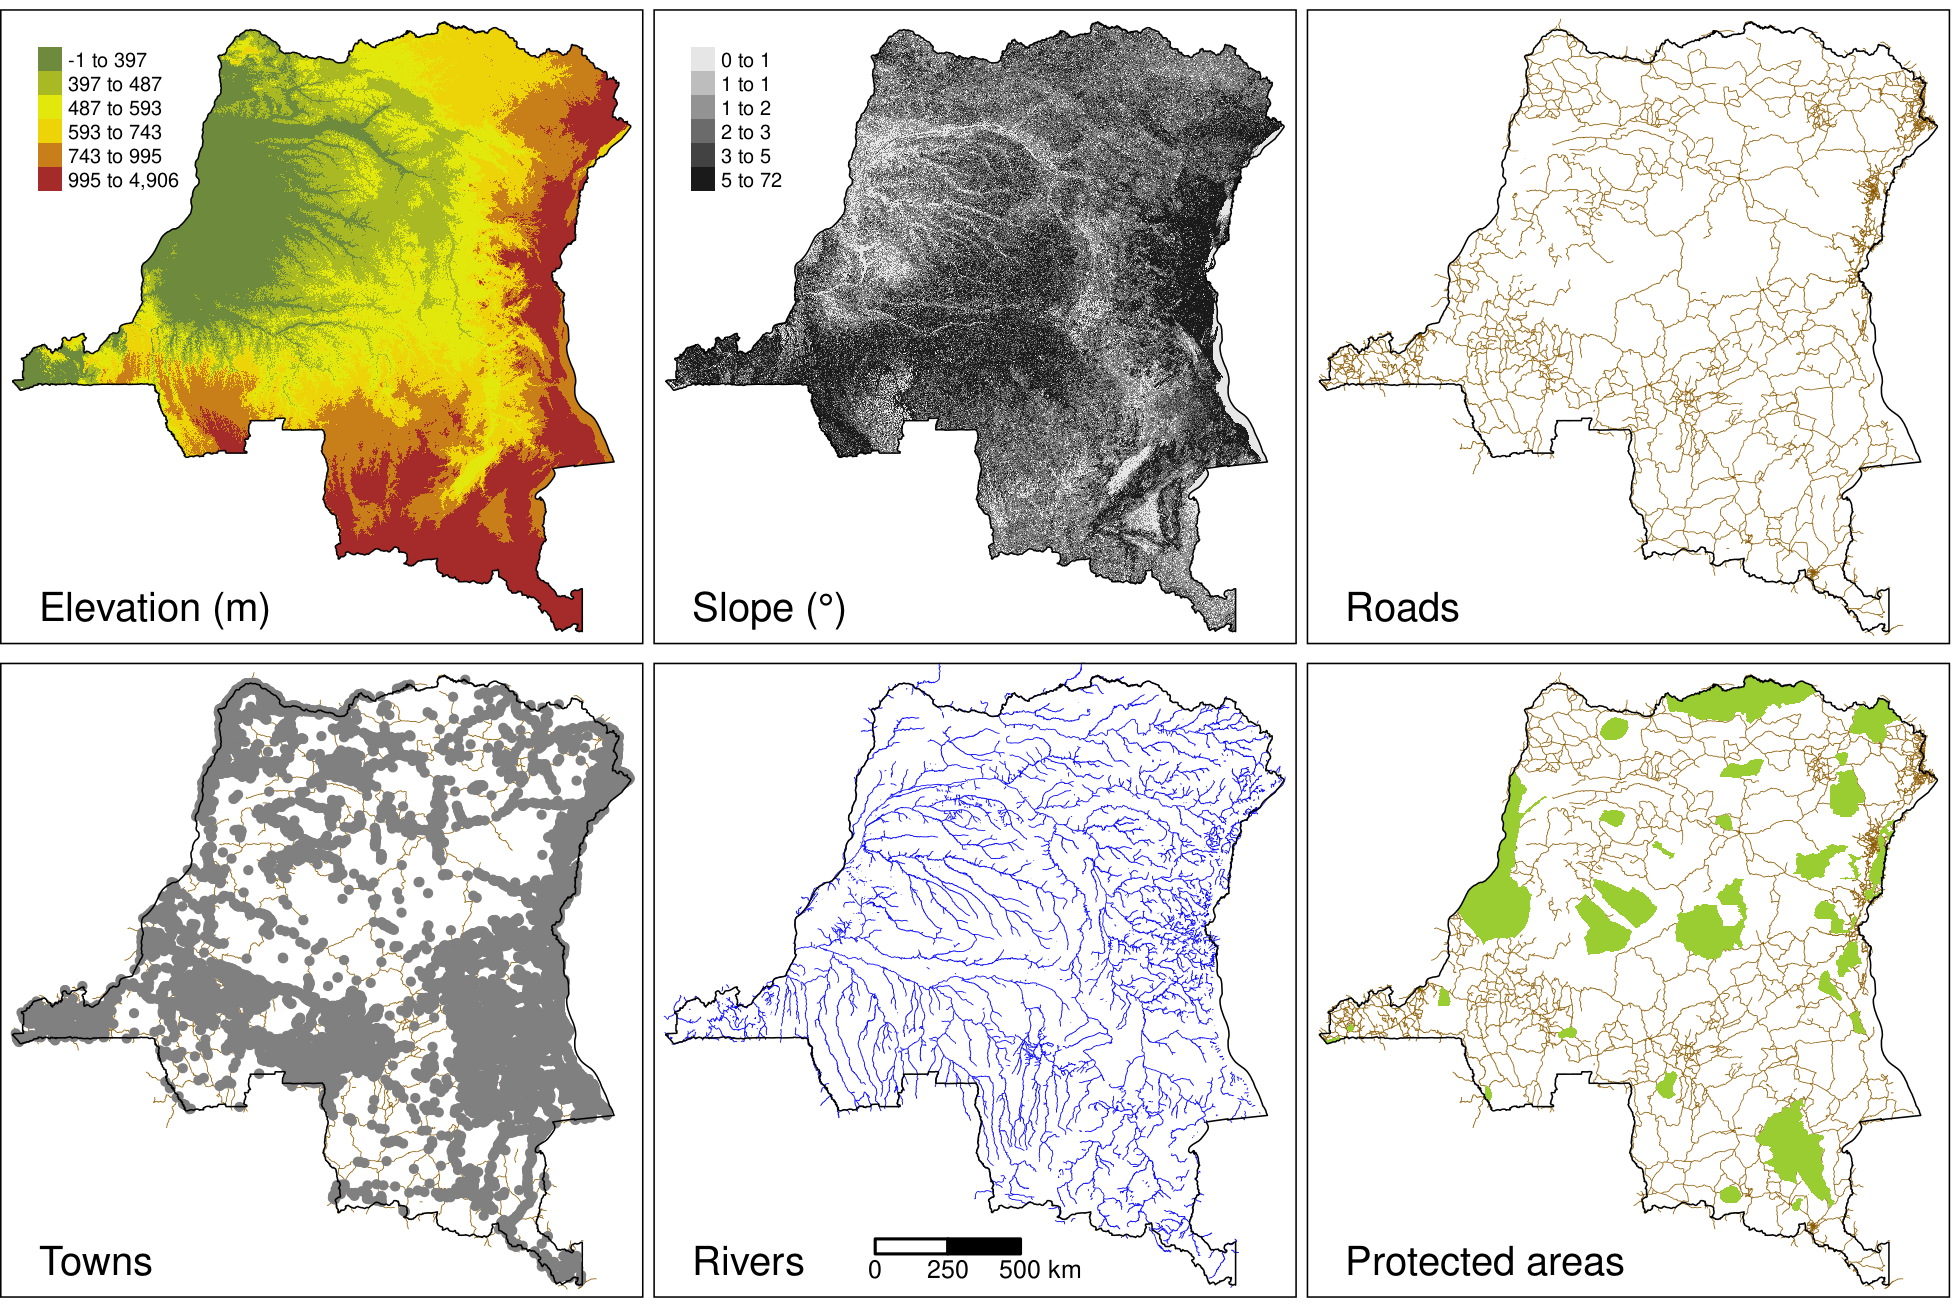
\includegraphics[width=0.8\textwidth]{figs/sm/var}

\structure{Spatial explanatory variables in DRC}
\end{frame}

\begin{frame}[label={sec:org854e294}]{Roads}
\begin{itemize}
\item OpenStreetMap (OSM)
\item ``motorway'', ``trunk'', ``primary'', ``secondary'' and ``tertiary'' roads
\item 3.6 million roads from OSM
\end{itemize}

\centering 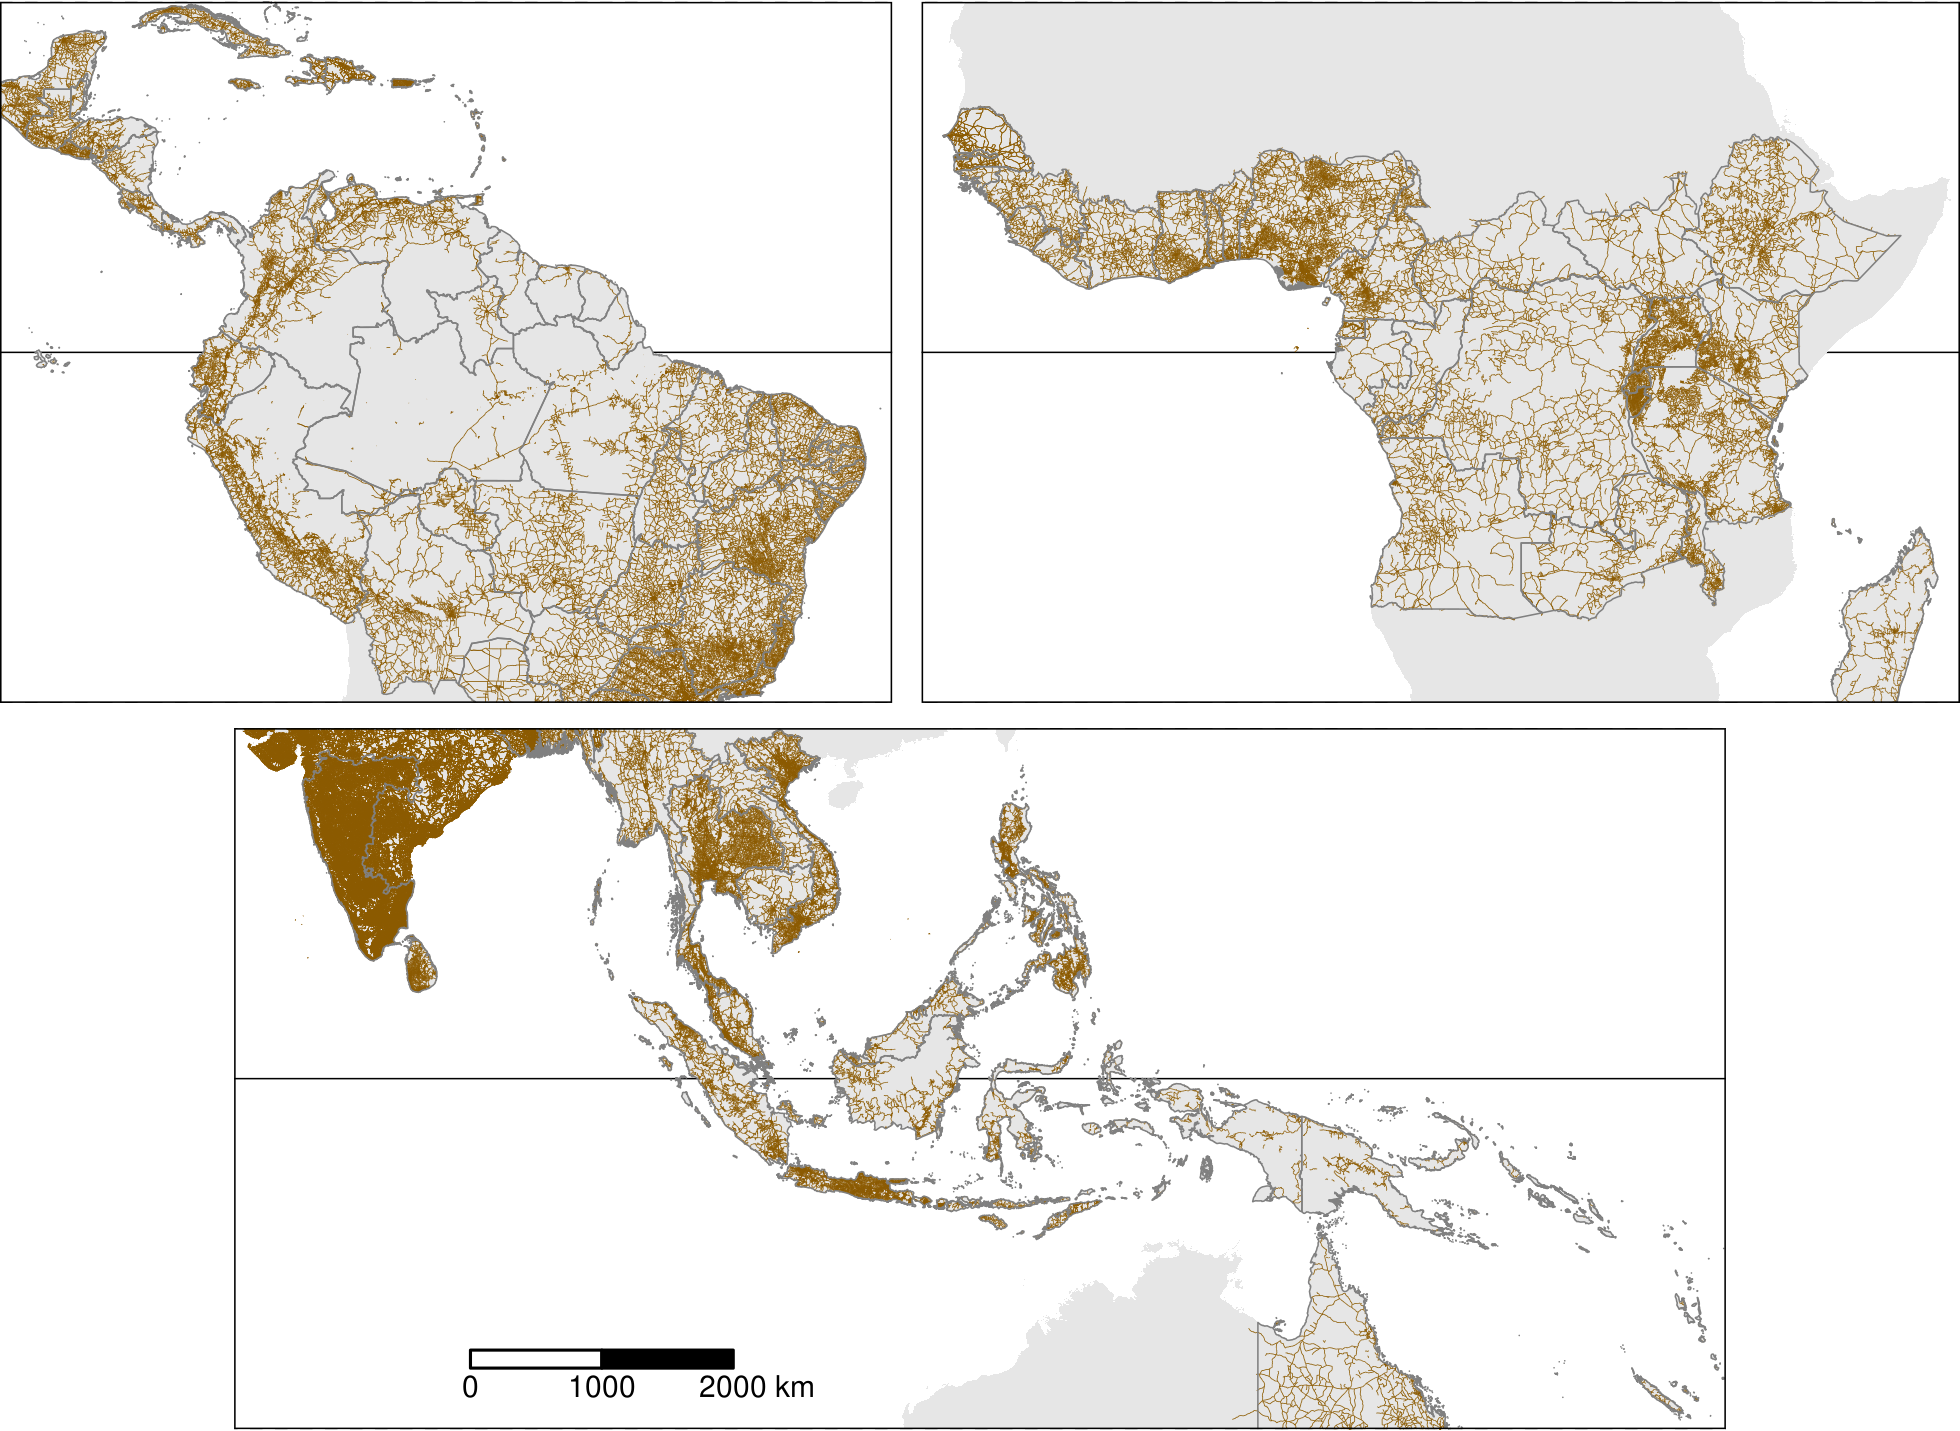
\includegraphics[width=0.7\textwidth]{figs/sm/roads}
\end{frame}

\begin{frame}[label={sec:org473f583}]{Protected areas}
\begin{itemize}
\item PA status: ``Designated'', ``Inscribed'', ``Established'', or ``Proposed''
before 1\textsuperscript{st} January 2010
\item 85,000 protected areas from WDPA
\end{itemize}

\centering 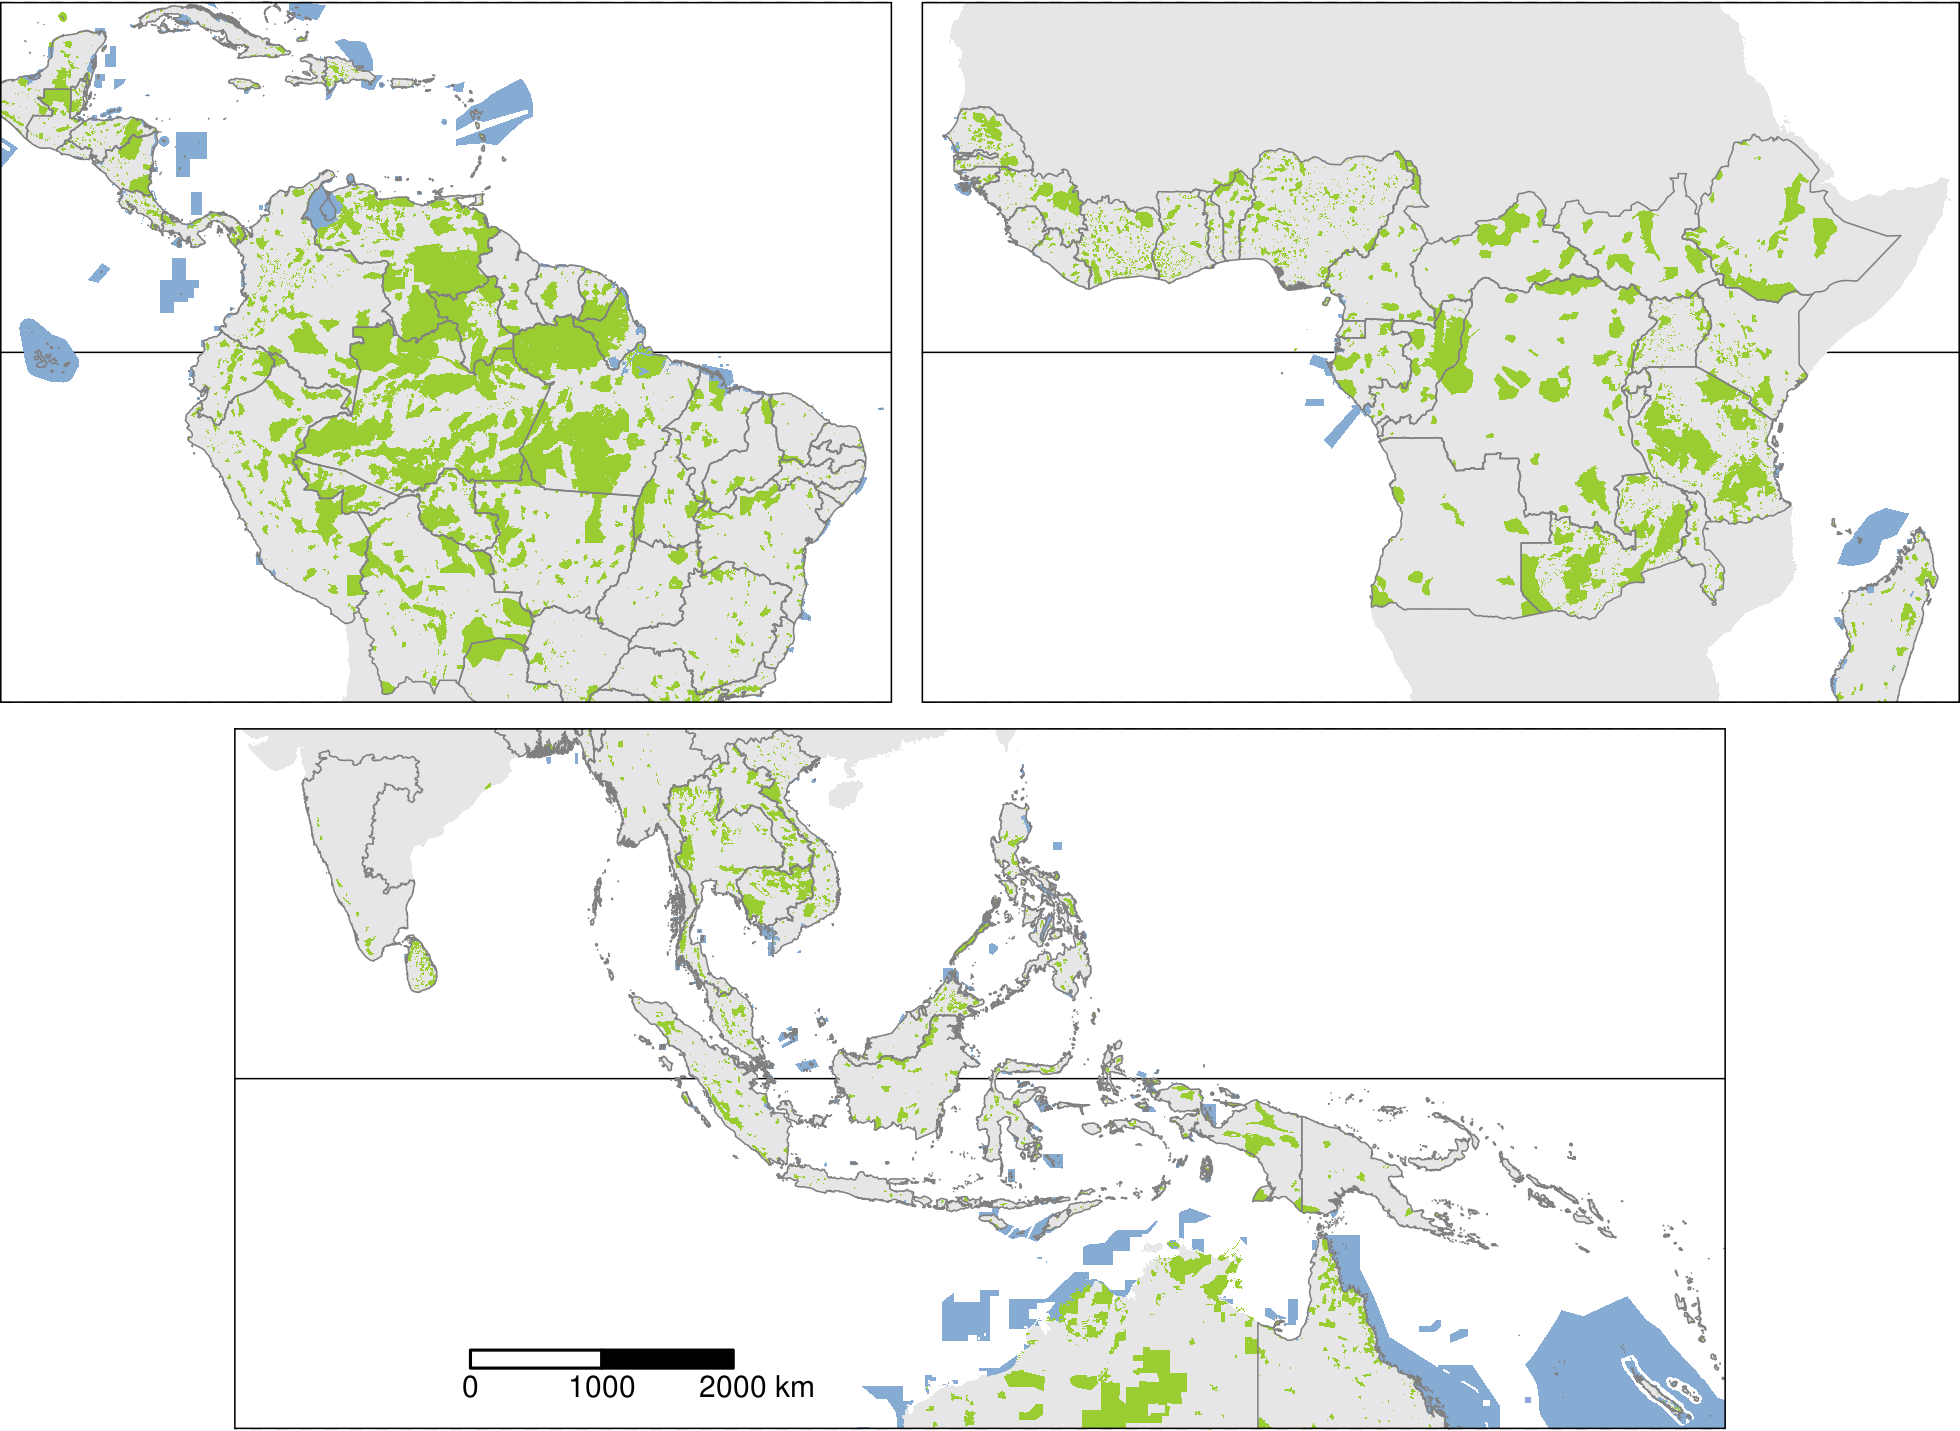
\includegraphics[width=0.7\textwidth]{figs/sm/pa}
\end{frame}

\begin{frame}[label={sec:org5a93361}]{Sampling}
\begin{itemize}
\item Stratified sampling between deforested/non-deforested pixels in
2010--2020
\item Total number of points proportional to the forest cover in 2010 (from
20,000 to 100,000 points per study area)
\end{itemize}

\centering 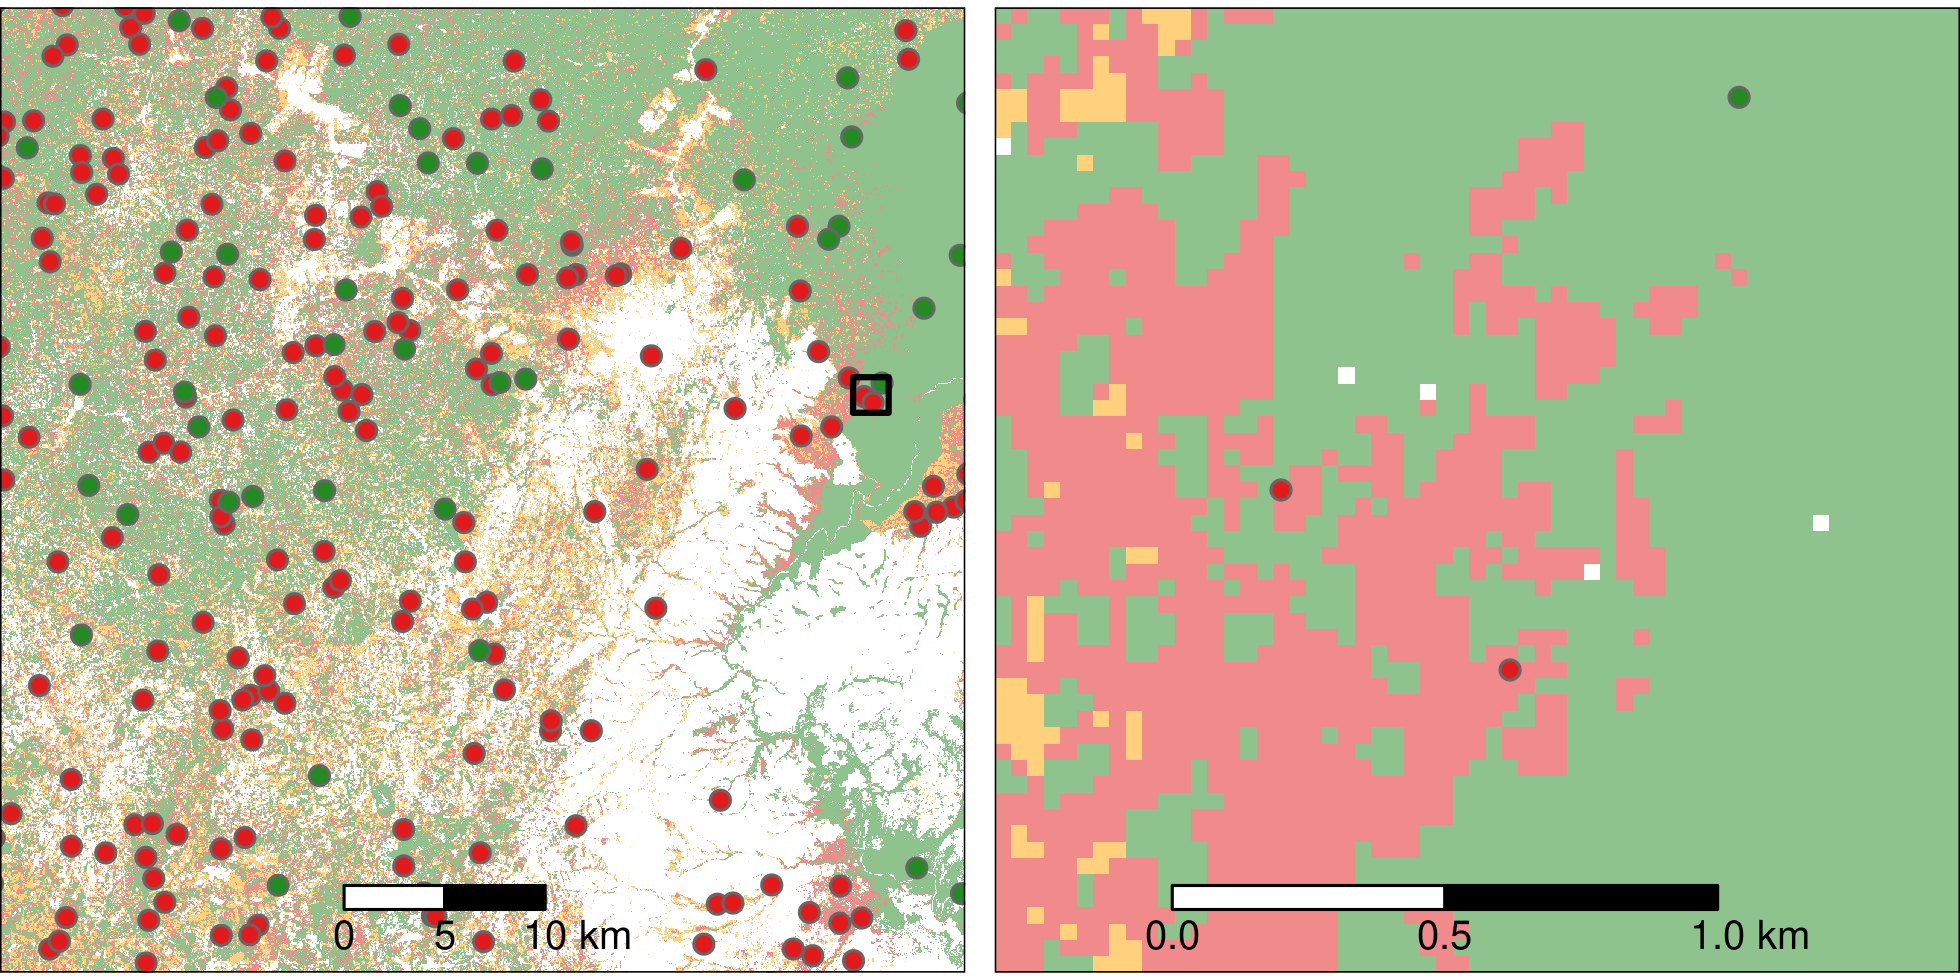
\includegraphics[width=0.7\textwidth]{figs/sm/sample.png}
\end{frame}

\subsection{Models}
\label{sec:orgb4a935e}
\begin{frame}[label={sec:orga07a282}]{Spatial risk of deforestation}
\begin{columns}
\begin{column}{0.5\columnwidth}
A logistic regression model with iCAR process

\begin{equation*}
\begin{split}
  y_i \sim \mathcal{B}ernoulli(\theta_i)\\
  \text{logit}(\theta_i) = \alpha + X_i \beta + \rho_{j(i)}\\
  \rho_{j(i)} \sim \mathcal{N}ormal(\sum_{j^{\prime}} \rho_{j^{\prime}} / n_j,V_{\rho} / n_j)
\end{split}
\end{equation*}

\footnotesize (NB: We can compare this model with a simple GLM and a Random
Forest model using a cross-validation procedure)
\end{column}

\begin{column}{0.5\columnwidth}
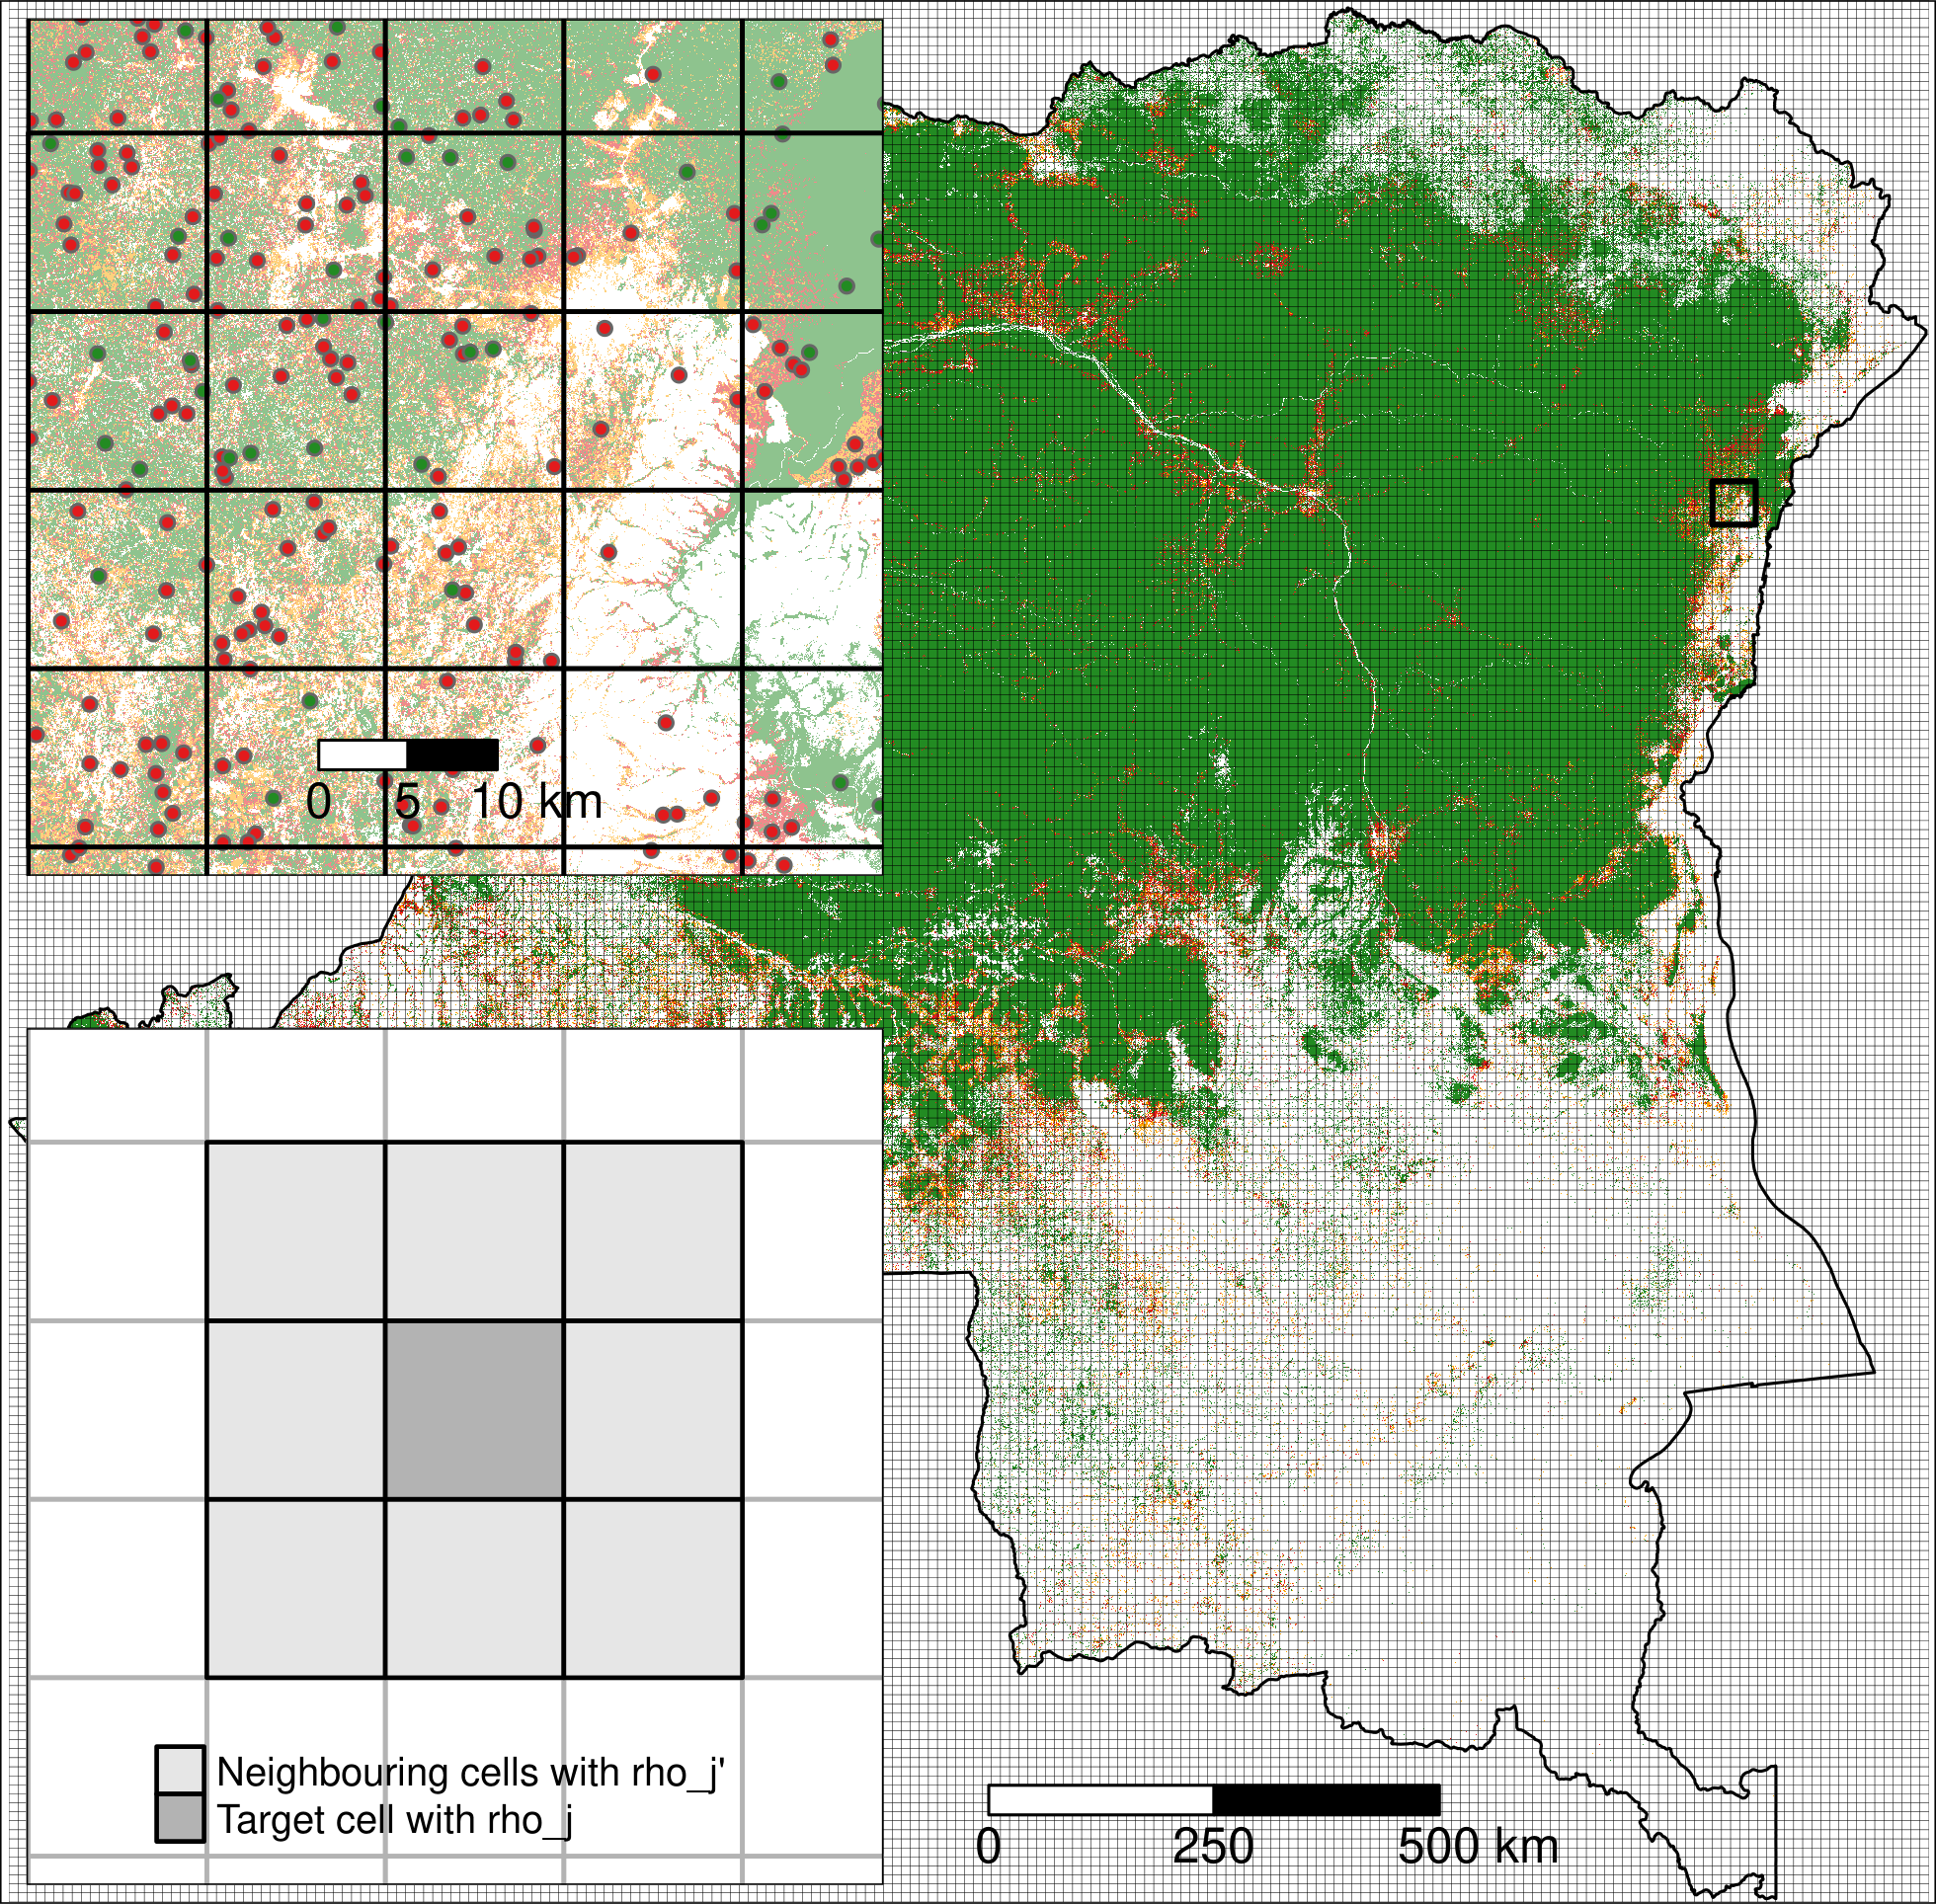
\includegraphics[width=\textwidth]{figs/sm/grid}

\structure{Square grid of 10km cells over DRC}
\end{column}
\end{columns}
\end{frame}

\subsection{Forecast}
\label{sec:org72e7afe}
\begin{frame}[label={sec:orgdcd5316}]{Spatial random effects}
\centering 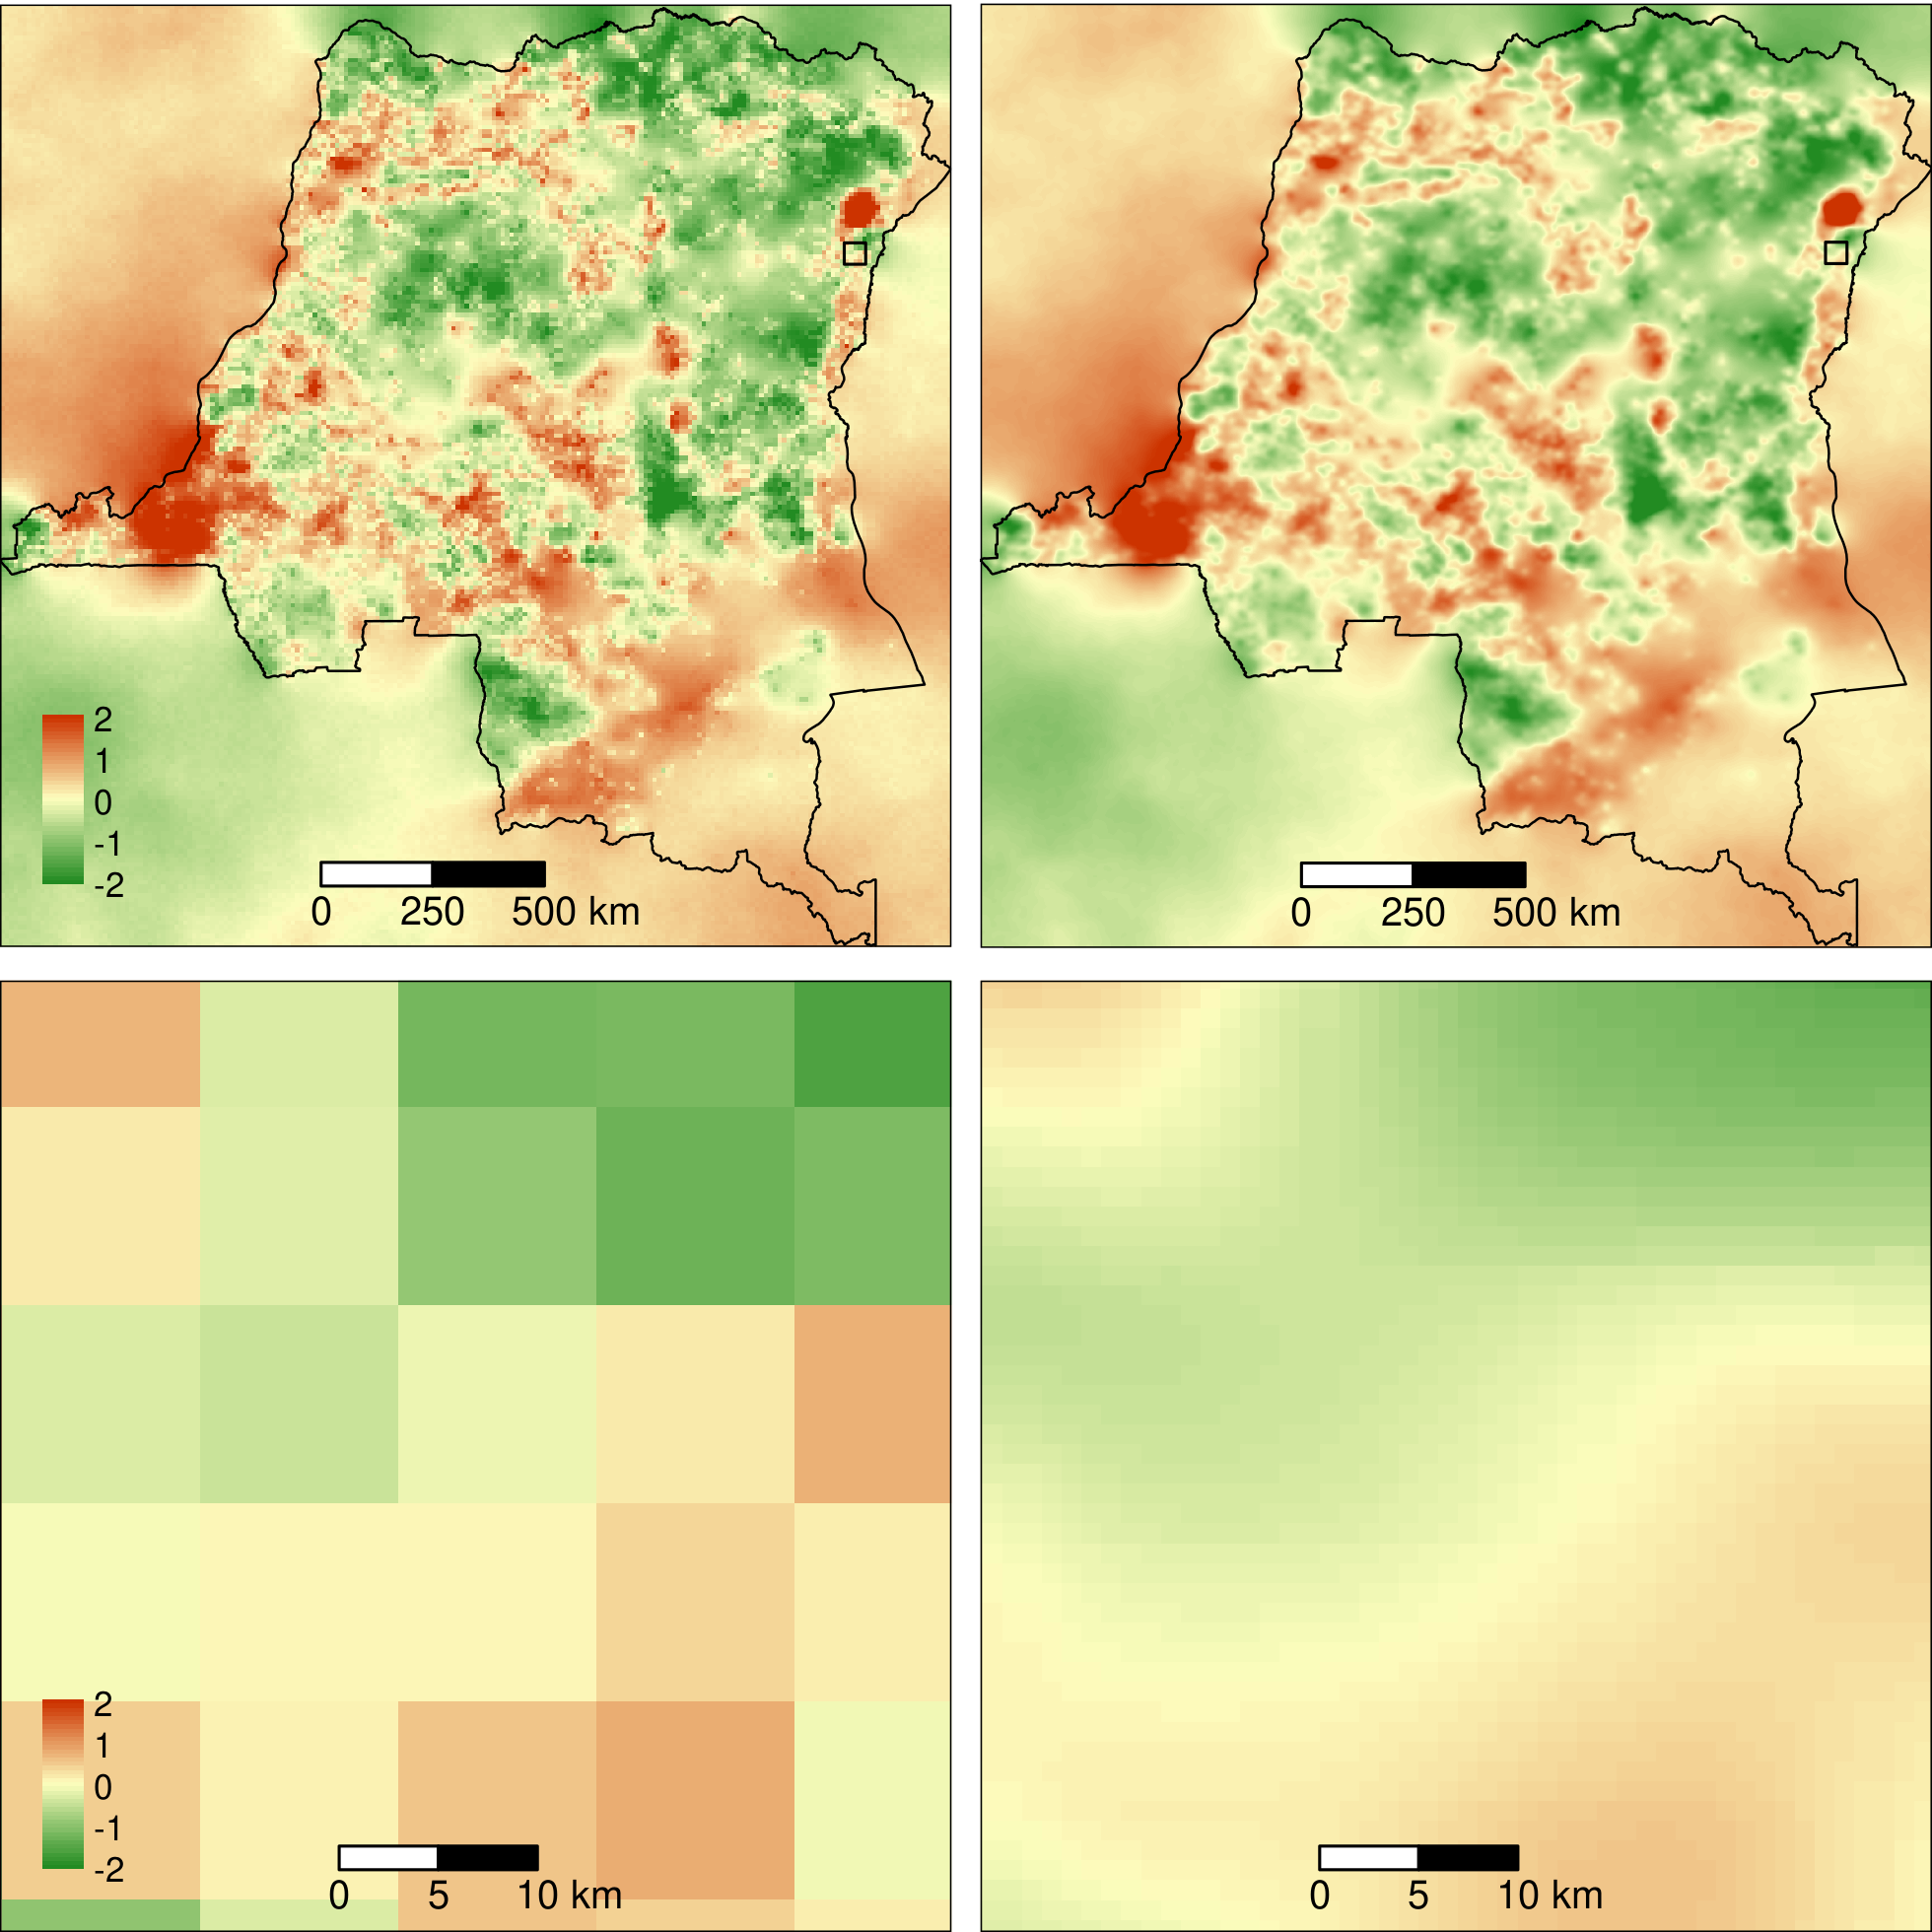
\includegraphics[width=0.6\textwidth]{figs/sm/rho.png}

\structure{Interpolation of spatial random effects at 1km in DRC}
\end{frame}

\begin{frame}[label={sec:org504fc2c}]{Spatial probability of deforestation}
We use the fitted model to compute the spatial probability of
deforestation.

\centering 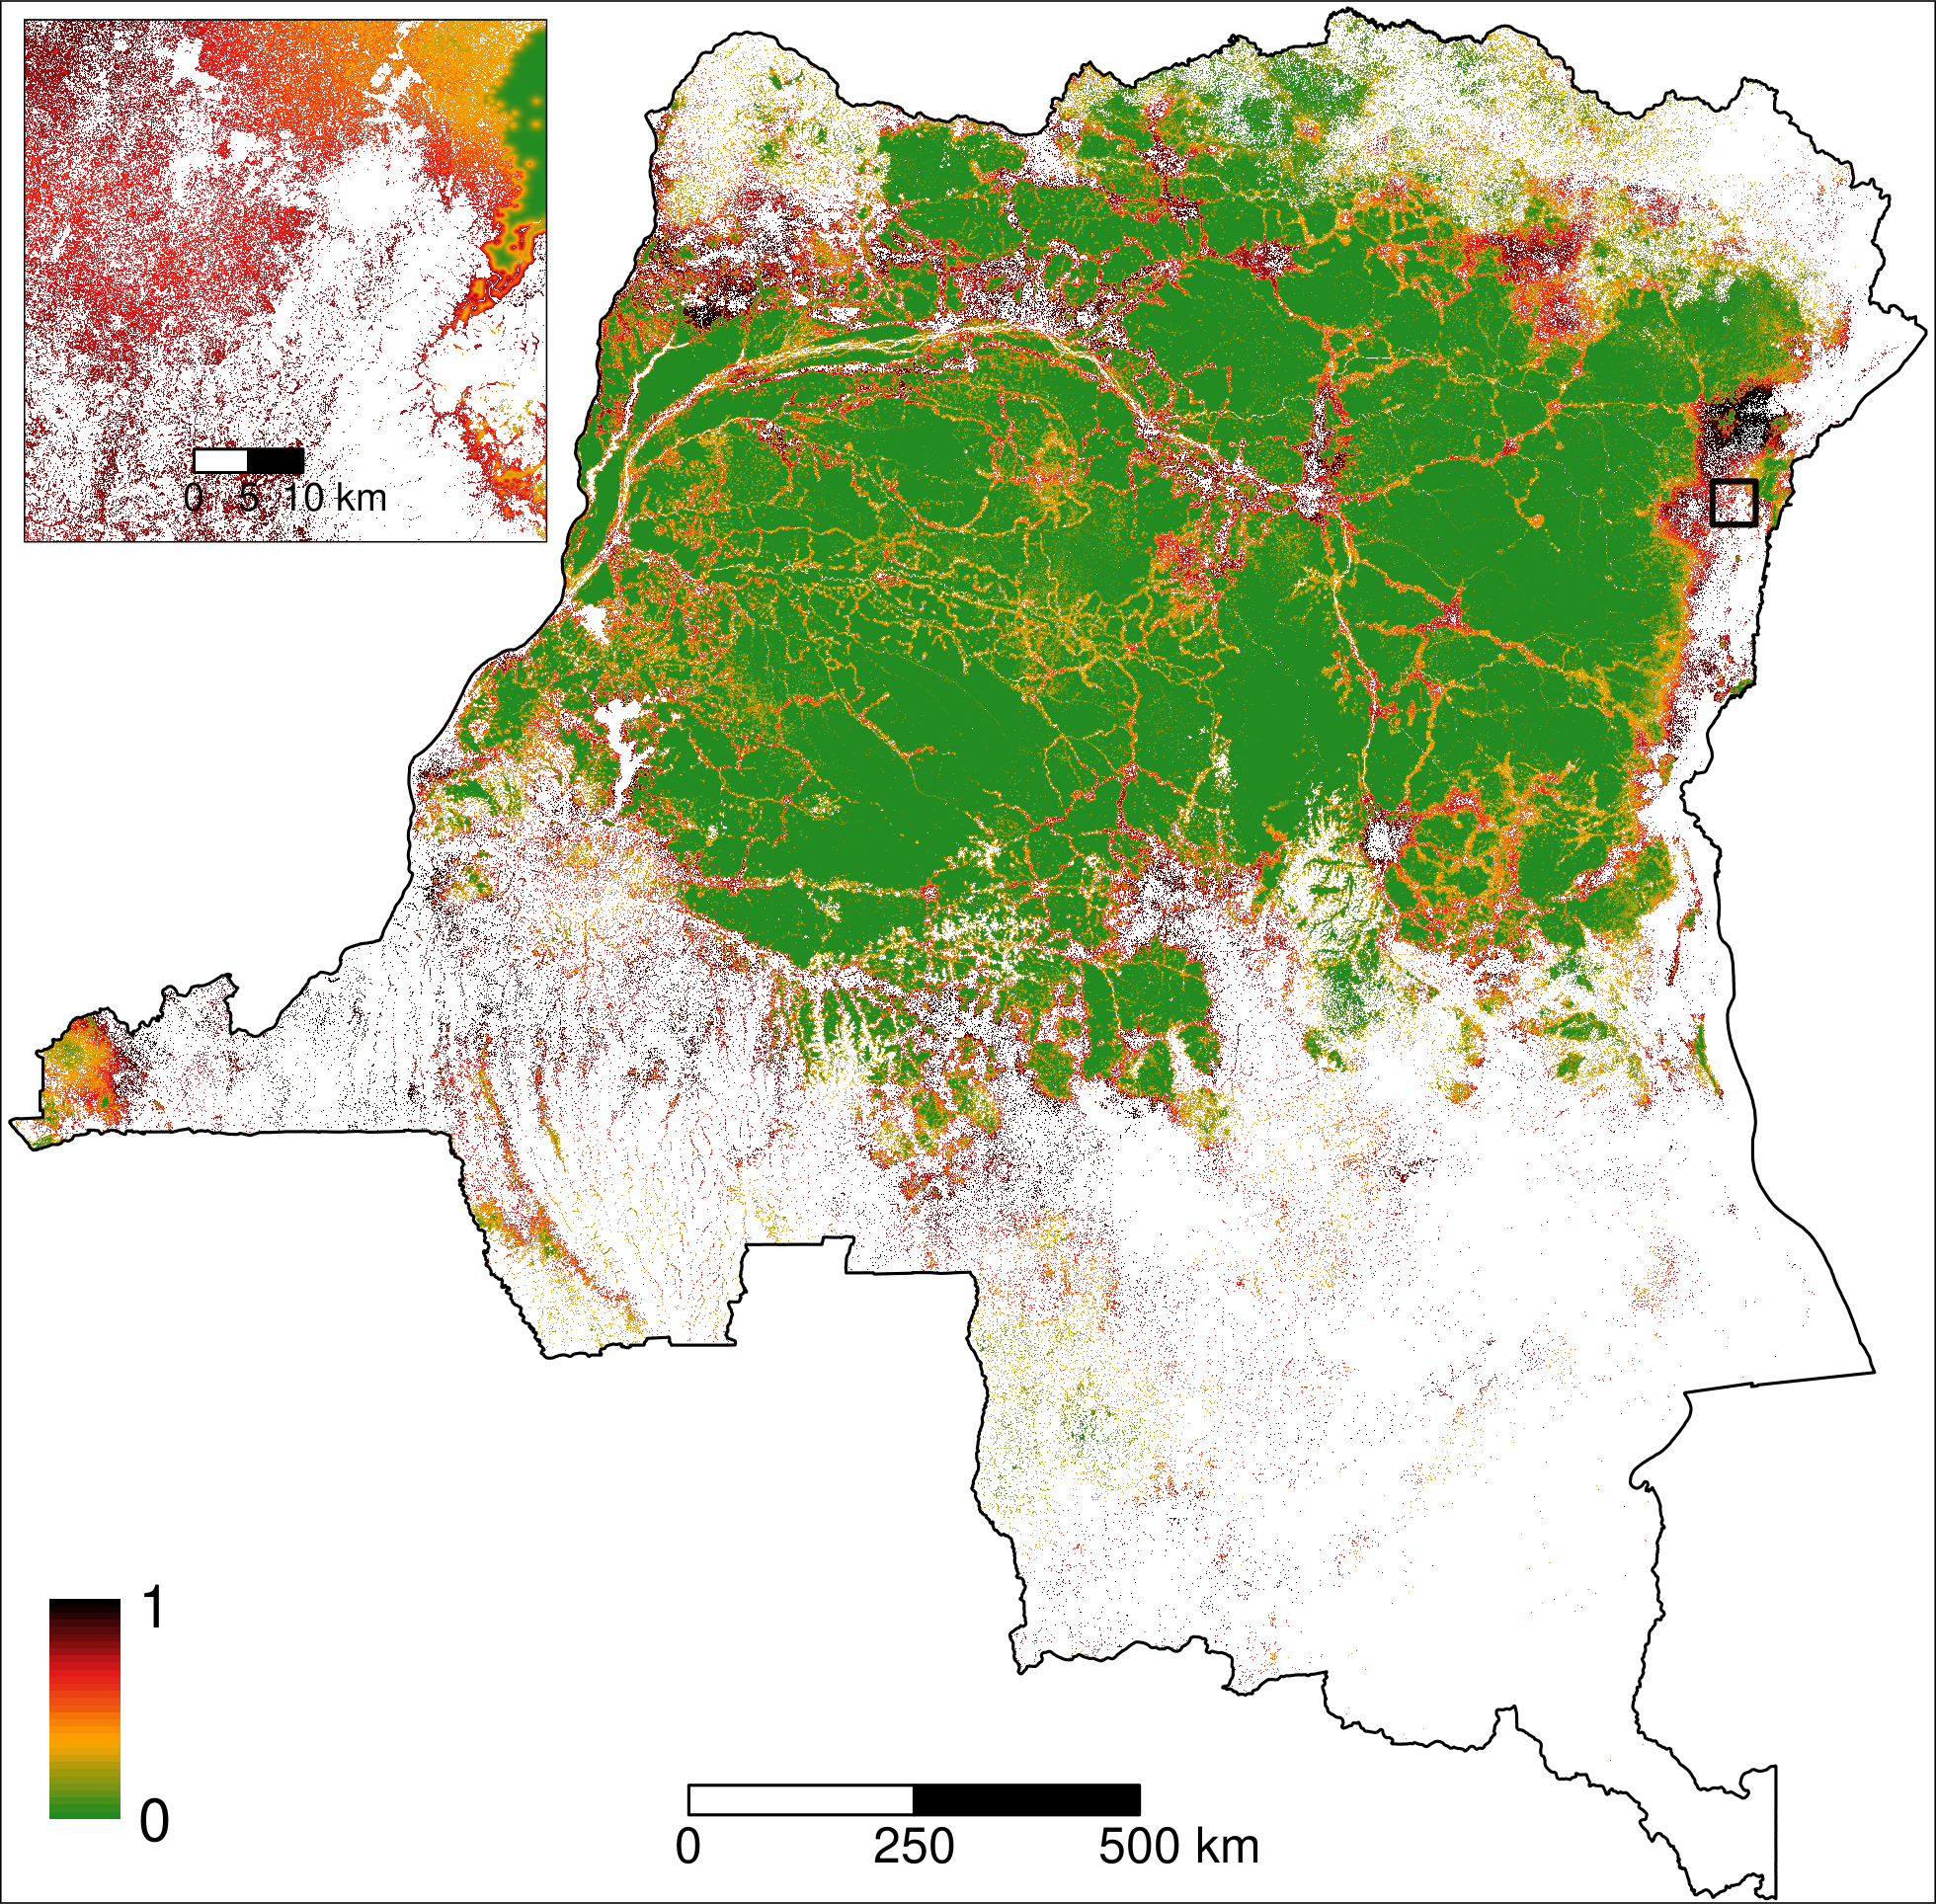
\includegraphics[width=0.5\textwidth]{figs/sm/prob.png}

\structure{Relative spatial probability of deforestation in DRC for the year 2020}
\end{frame}

\begin{frame}[label={sec:orgad5bffc}]{Future forest cover}
\begin{itemize}
\item \structure{Various deforestation scenarios can be considered}
\item Total deforested area \(D\) (ha) in a given period of time \(Y\) (yr).
\item Number of pixels to be deforested: \(n=D/\text{pixel area}\).
\item Deforestation \(n\) pixels with the highest deforestation probabilities.
\end{itemize}

\centering 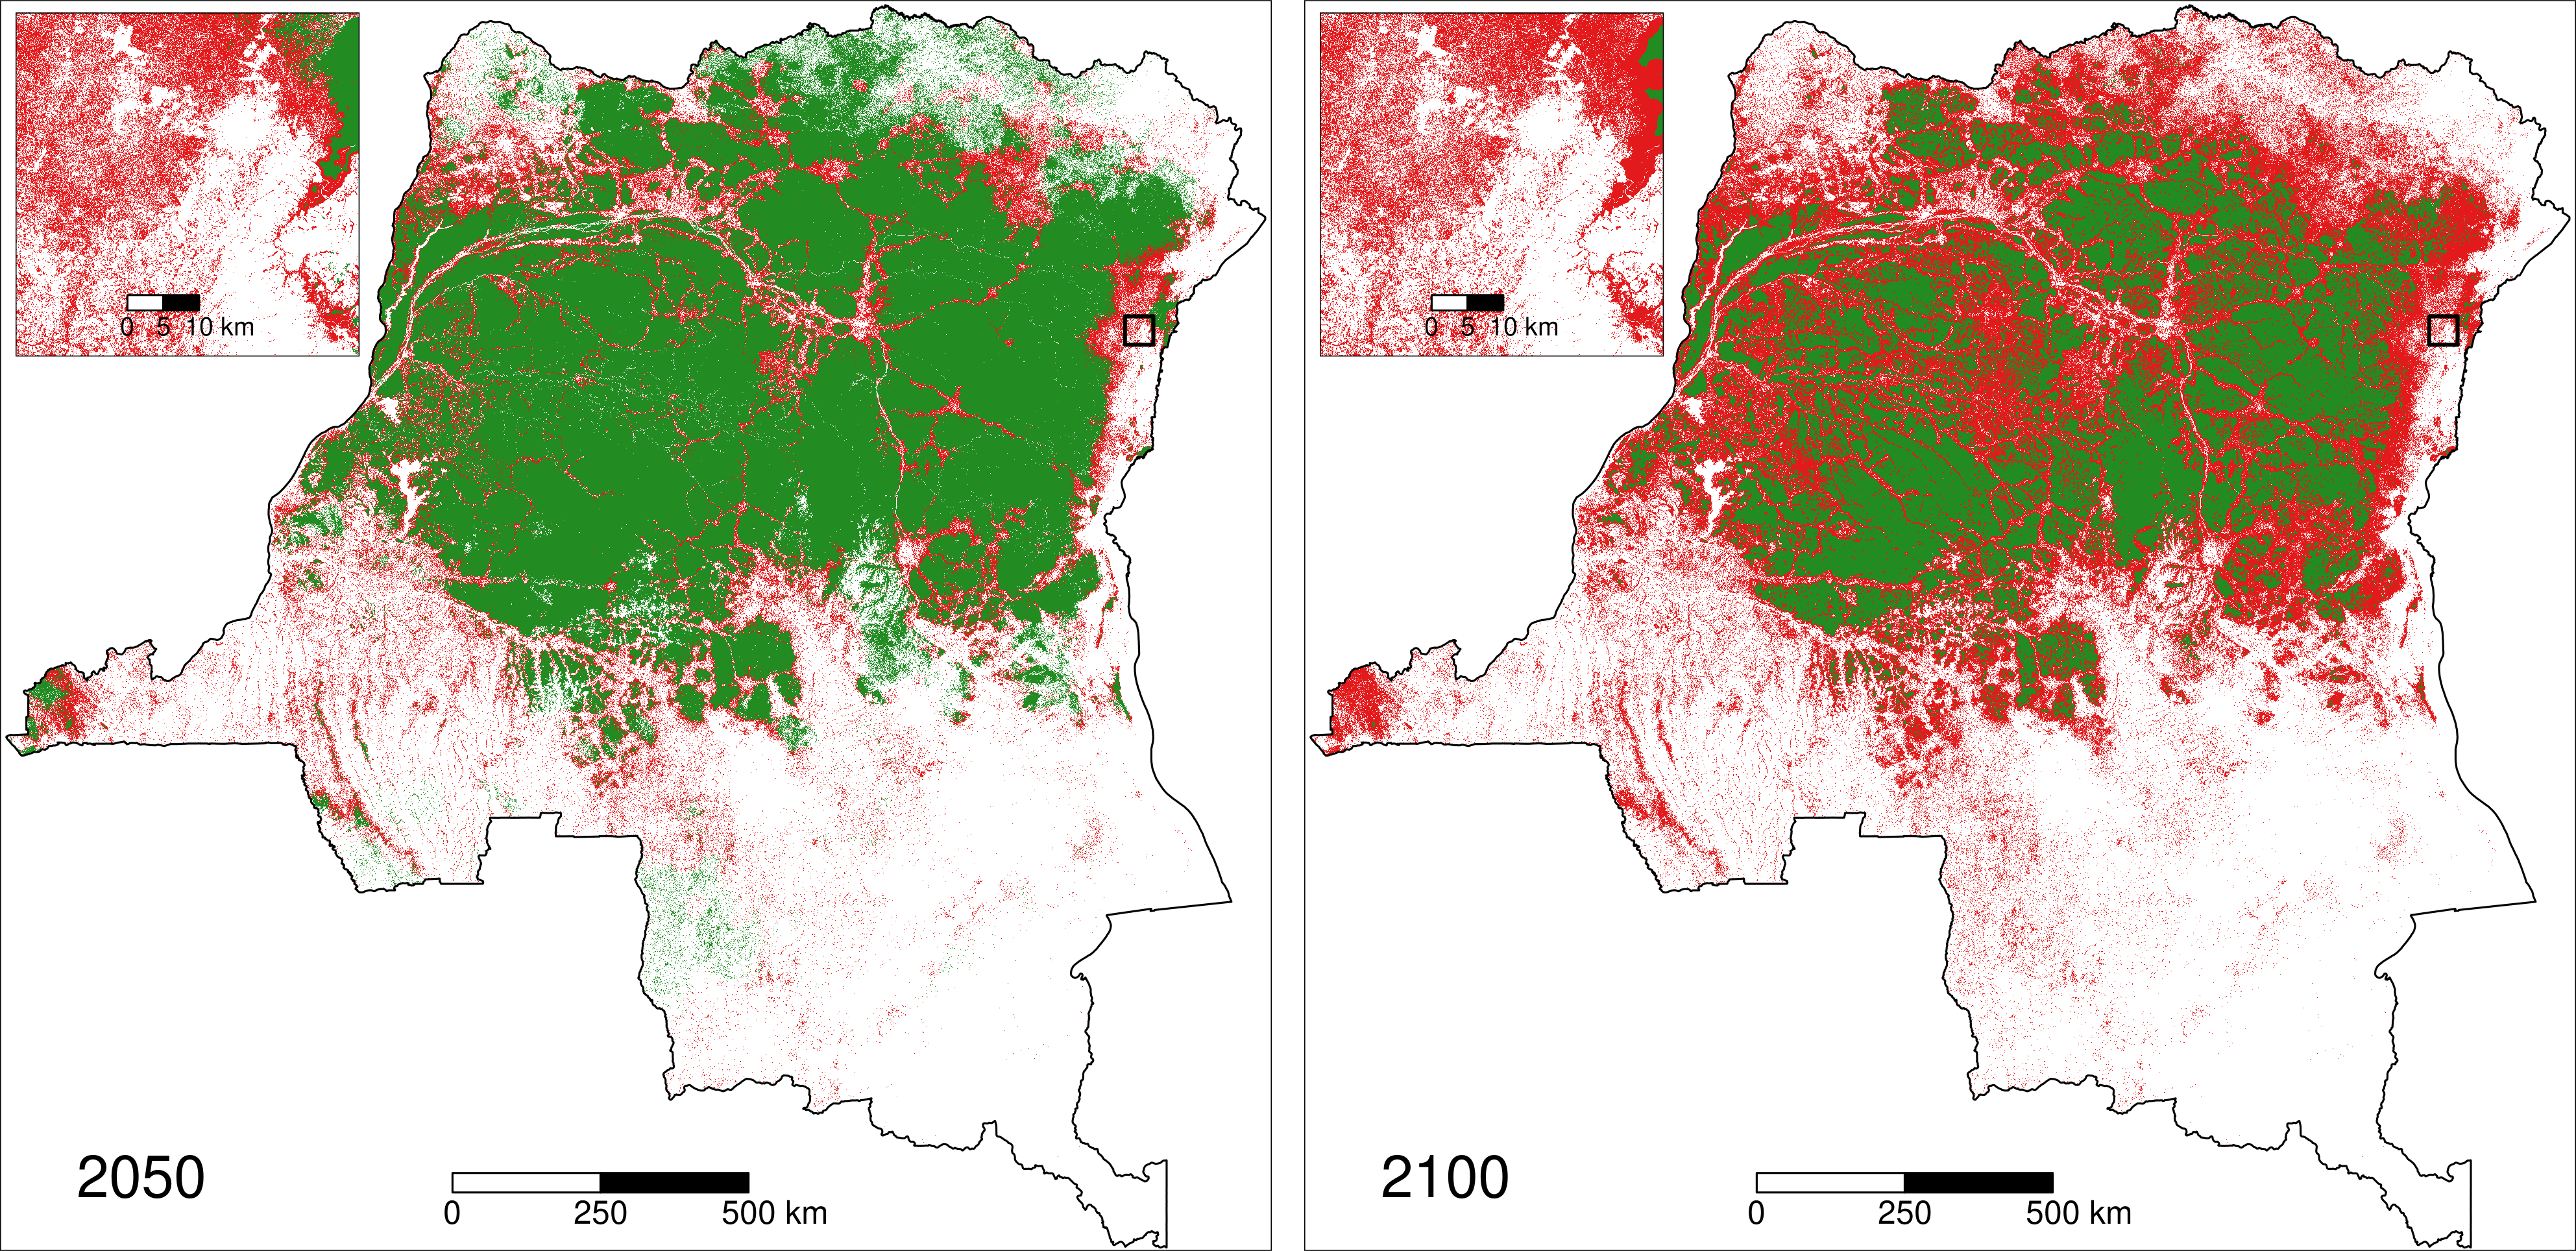
\includegraphics[width=0.7\textwidth]{figs/sm/fcc2050_2100.png}

\structure{Projected deforestation in 2020--2050 and 2020--2100 in DRC}
\end{frame}

\begin{frame}[label={sec:org1b9cc07}]{Future carbon emissions}
\begin{columns}
\begin{column}{0.5\columnwidth}
\begin{itemize}
\item We can combine the map of the projected deforestation with a forest carbon map to compute emissions.
\item Example for DRC with map by Avitabile et al. (2016) at 1km resolution.
\end{itemize}
\end{column}

\begin{column}{0.5\columnwidth}
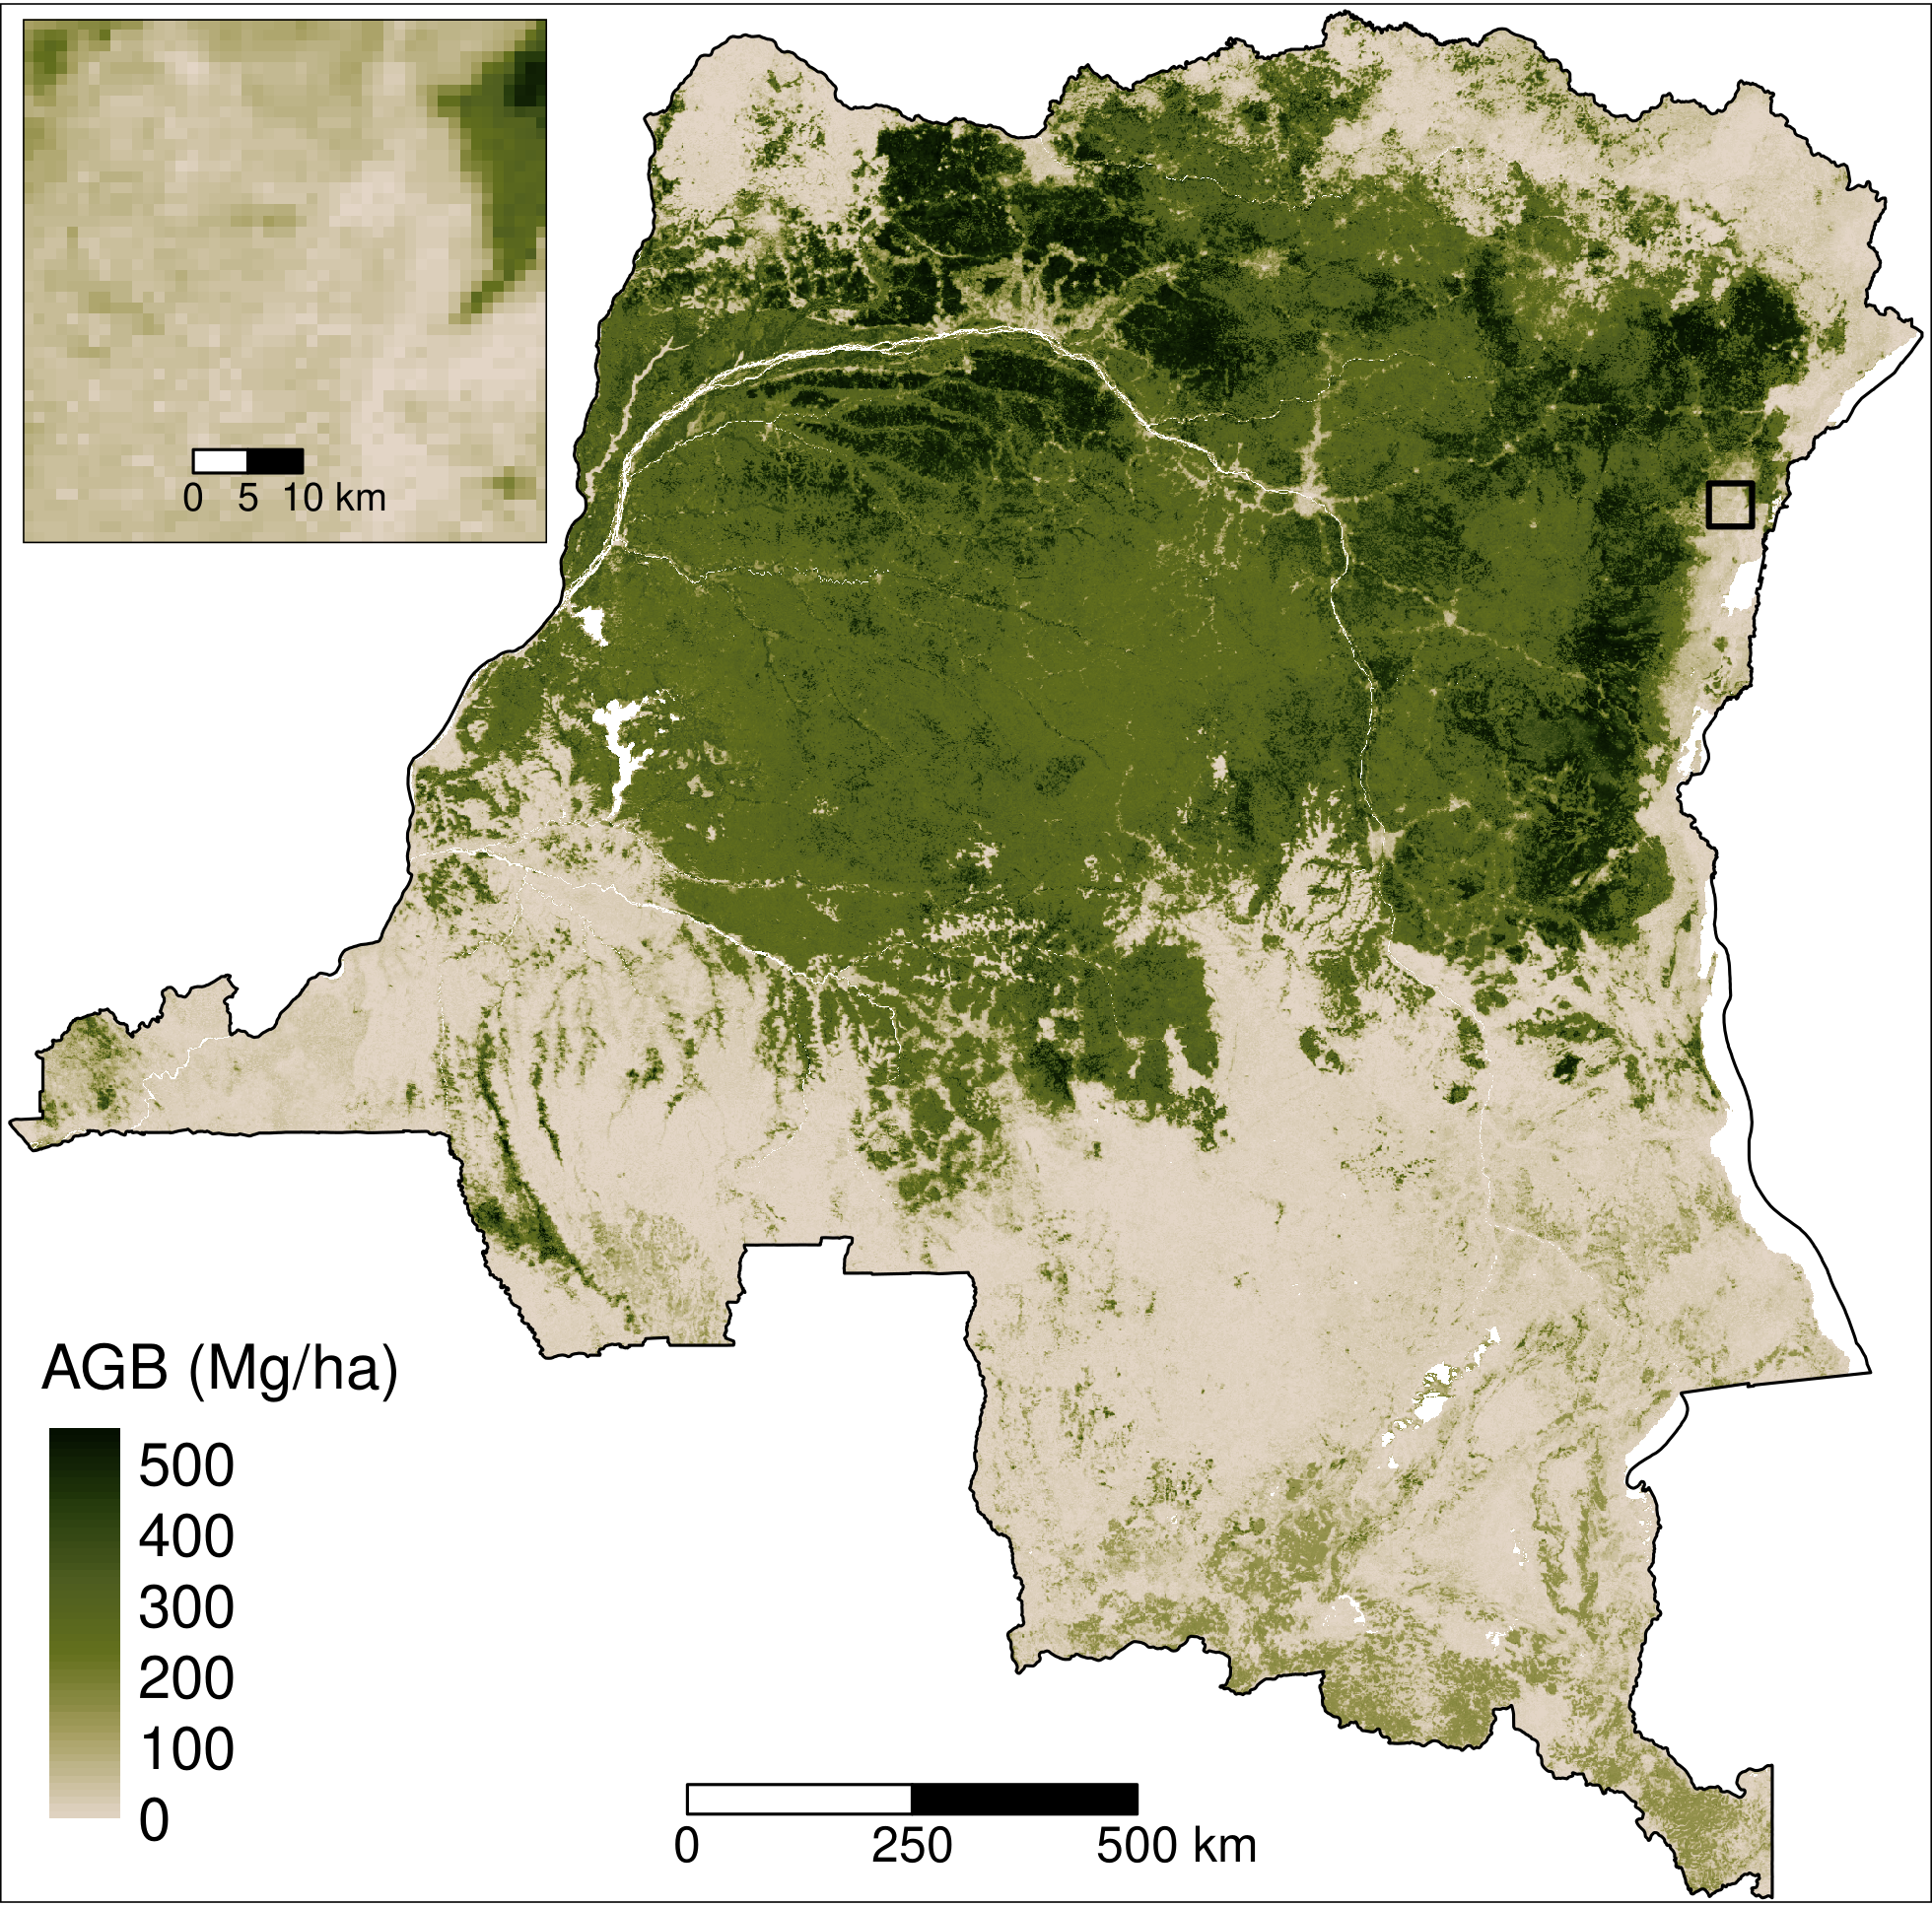
\includegraphics[width=\textwidth]{figs/sm/AGB}

\structure{Aboveground biomass in DRC}
\end{column}
\end{columns}
\end{frame}

\section{Applications}
\label{sec:orge02c9b1}
\subsection{ForestAtRisk in the tropics}
\label{sec:orgea4c3bb}
\begin{frame}[label={sec:orgaab9a35}]{Study areas}
\begin{itemize}
\item \structure{i.} Consider tropical moist forest in \structure{92} countries (119 study areas)
\item \structure{ii.} Estimate the current deforestation rate and uncertainty in each country
\item \structure{iii.} Model the spatial risk of deforestation from environmental factors
\item \structure{iv.} Forecast the deforestation assuming a business-as-usual scenario
\item \structure{v.} Consequences in terms of carbon emissions
\end{itemize}

\vspace{0.5cm}
\begin{center}
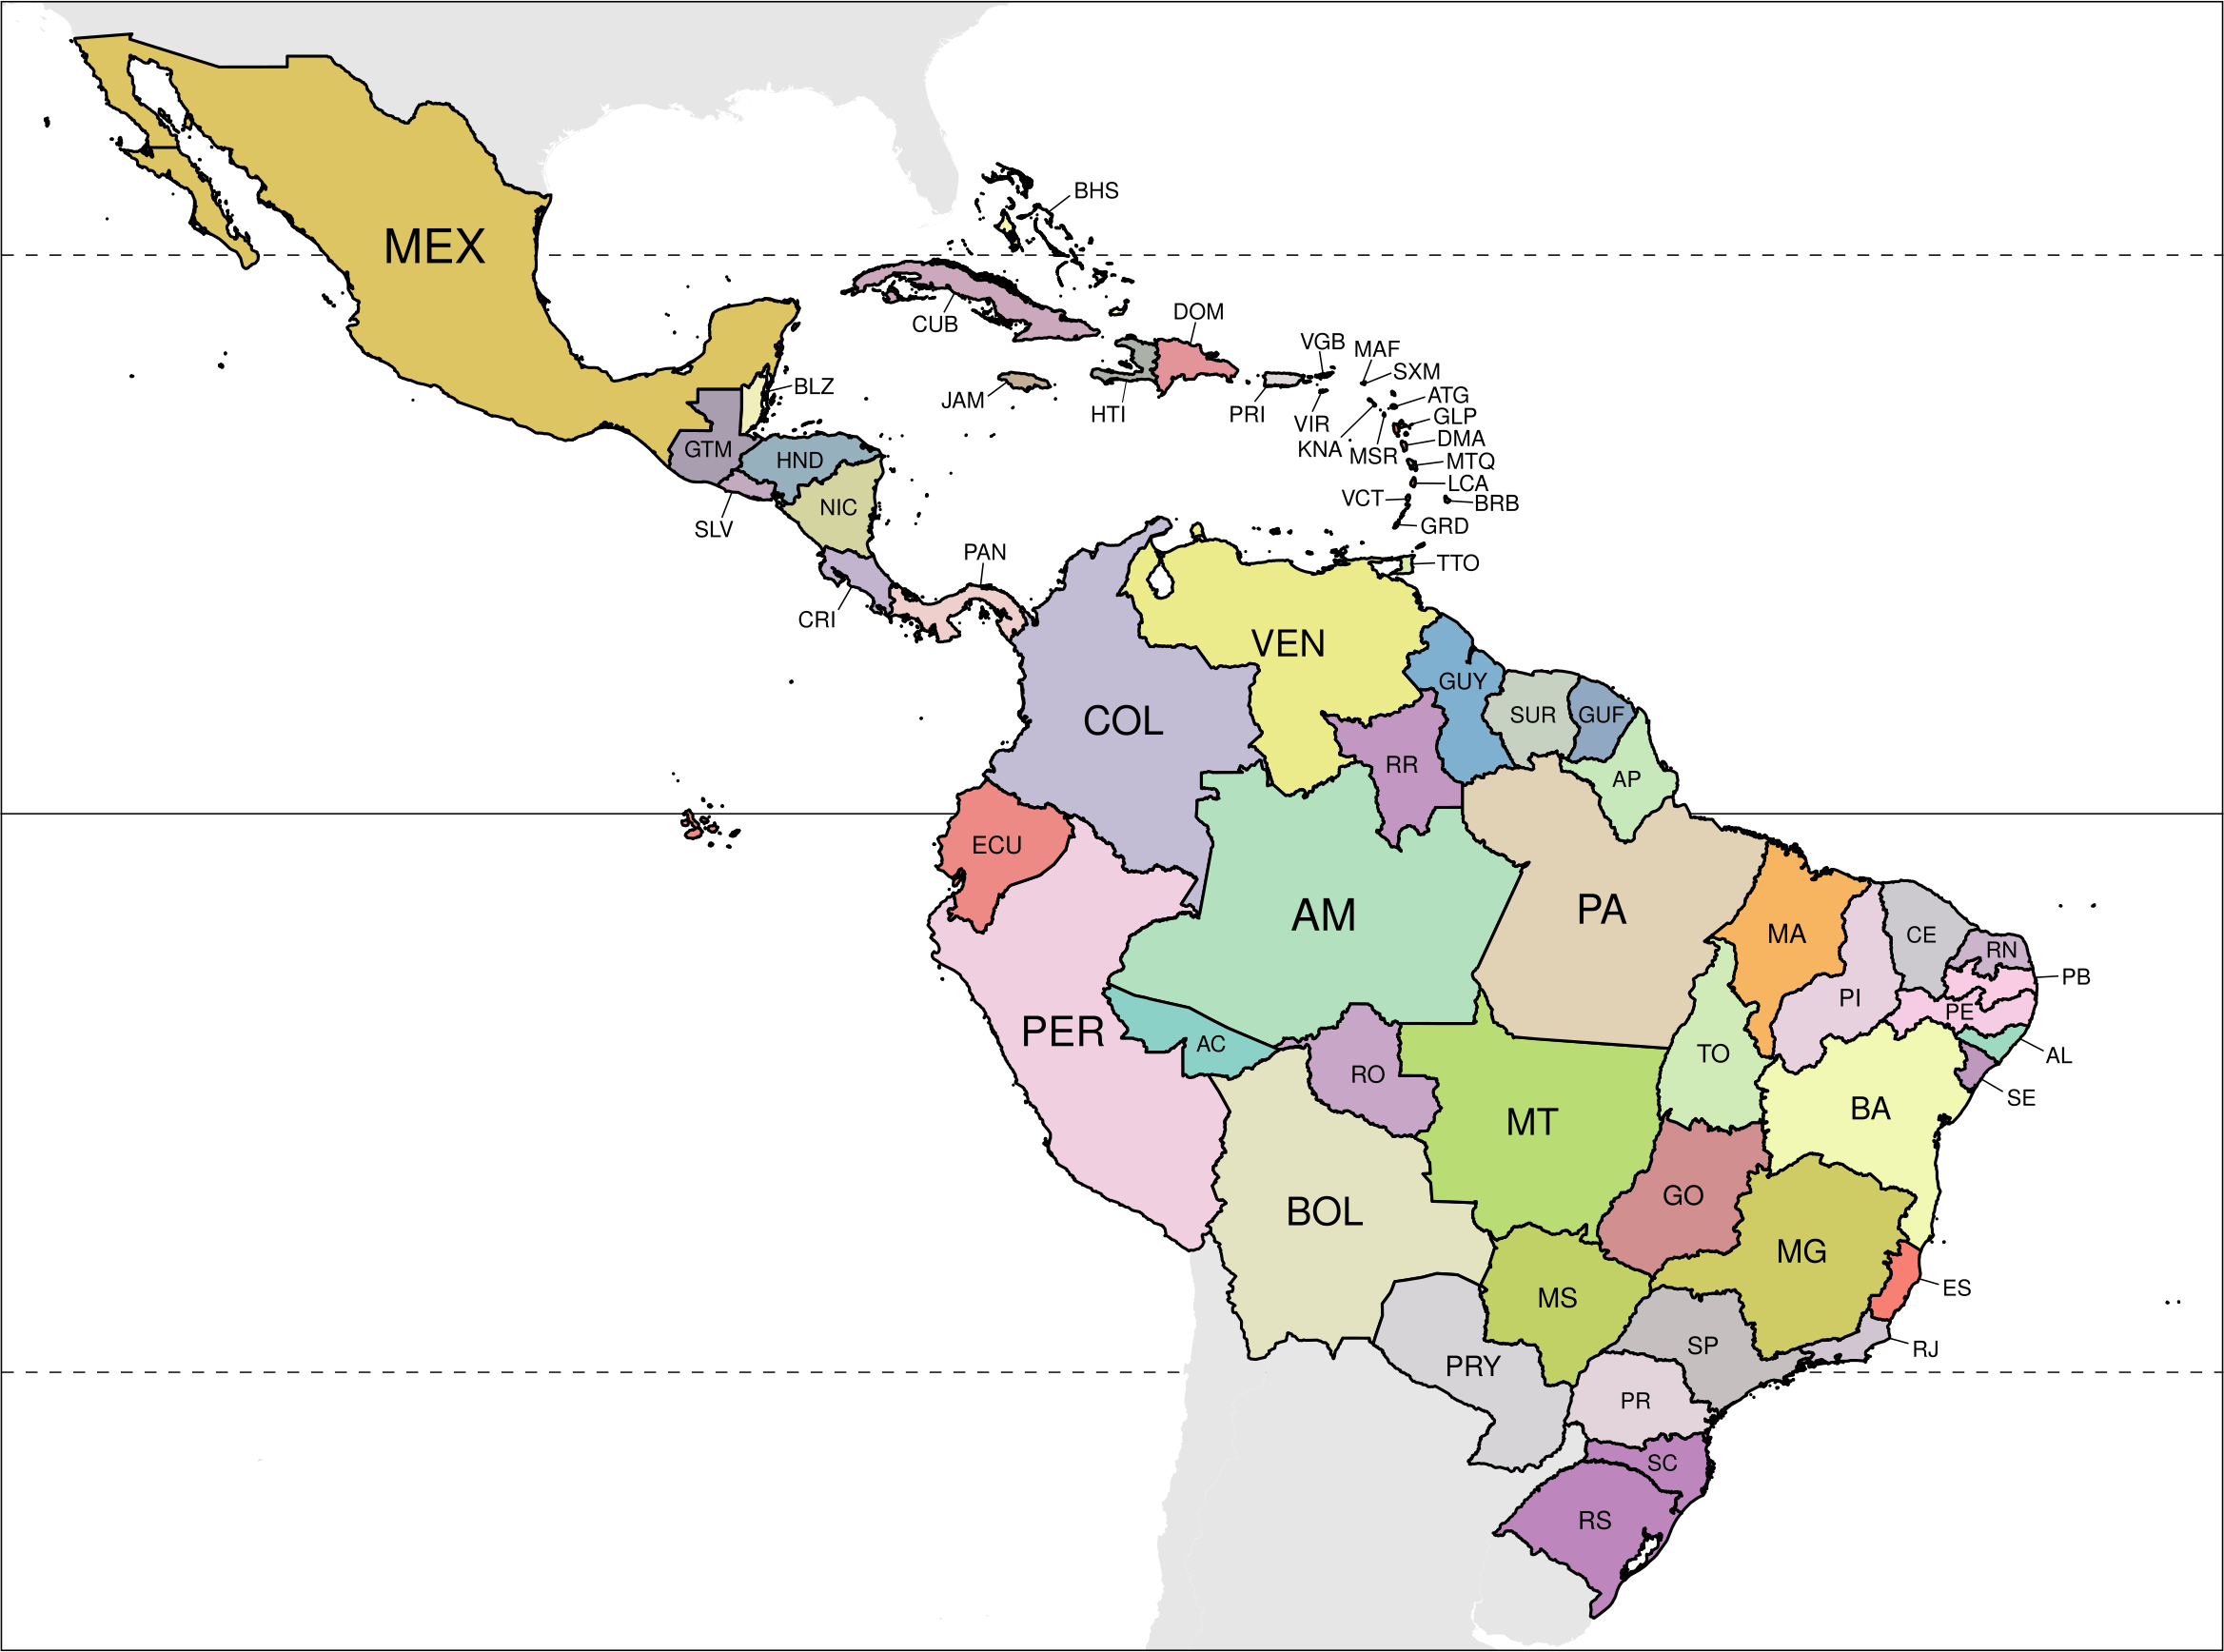
\includegraphics[width=0.32\textwidth]{figs/sm/study_areas_America}
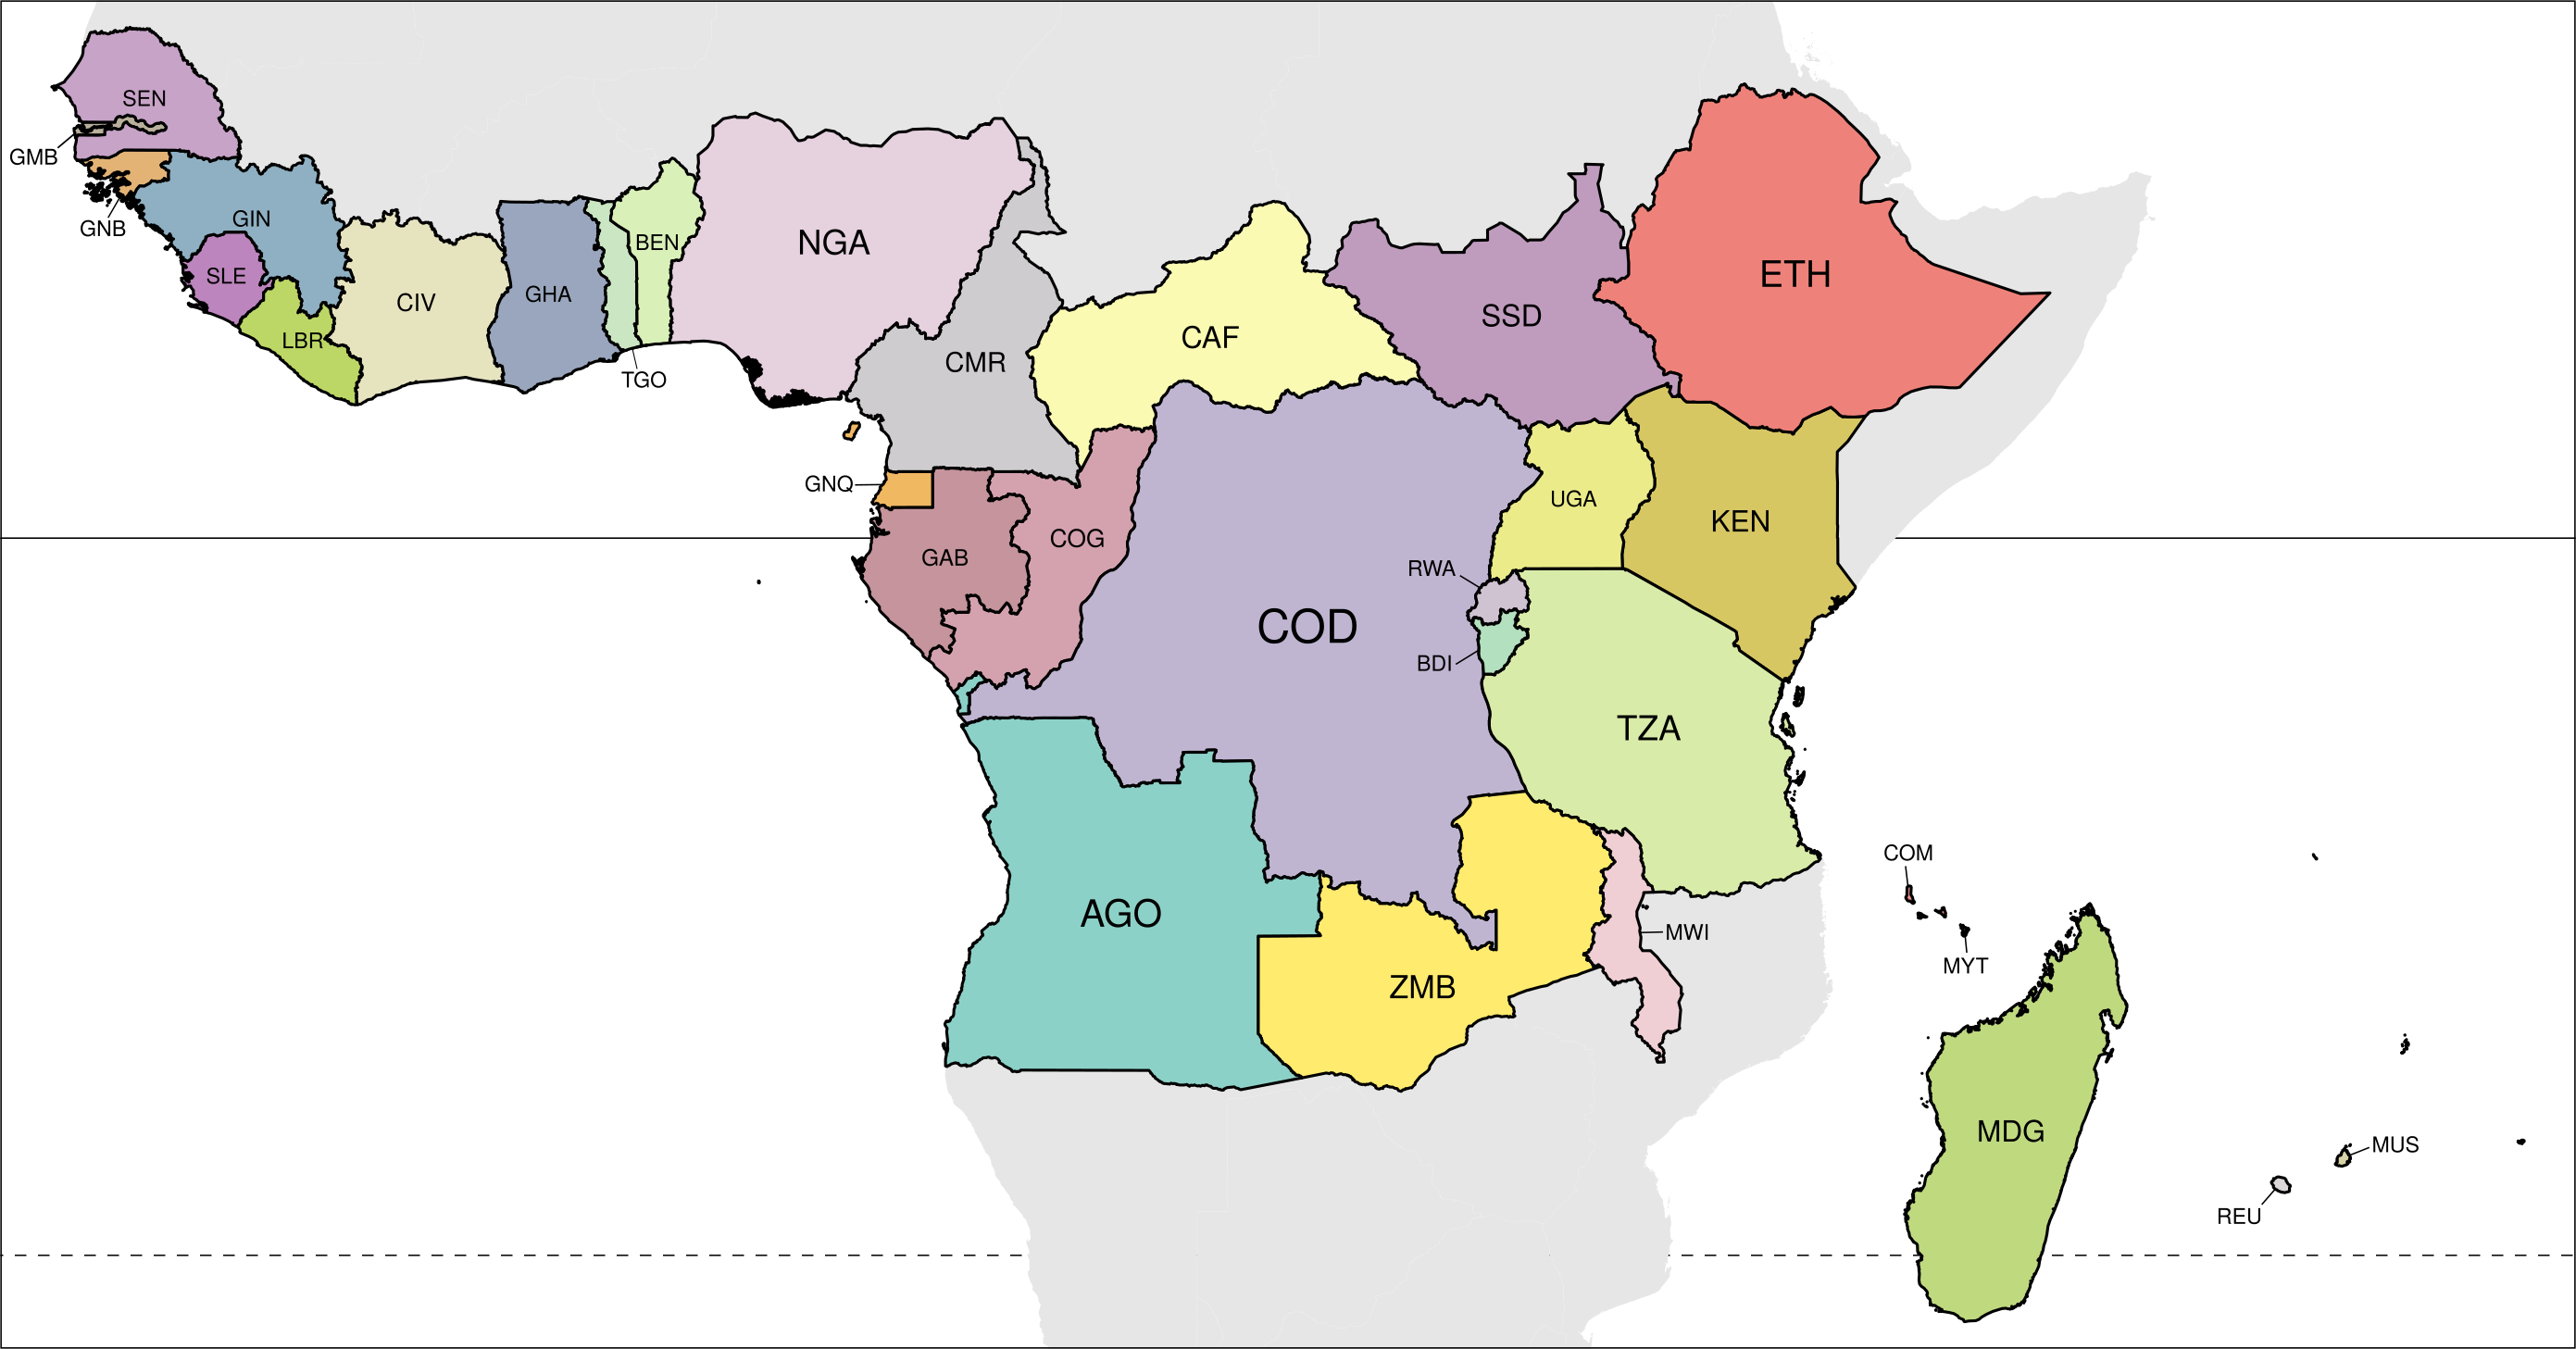
\includegraphics[width=0.32\textwidth]{figs/sm/study_areas_Africa}
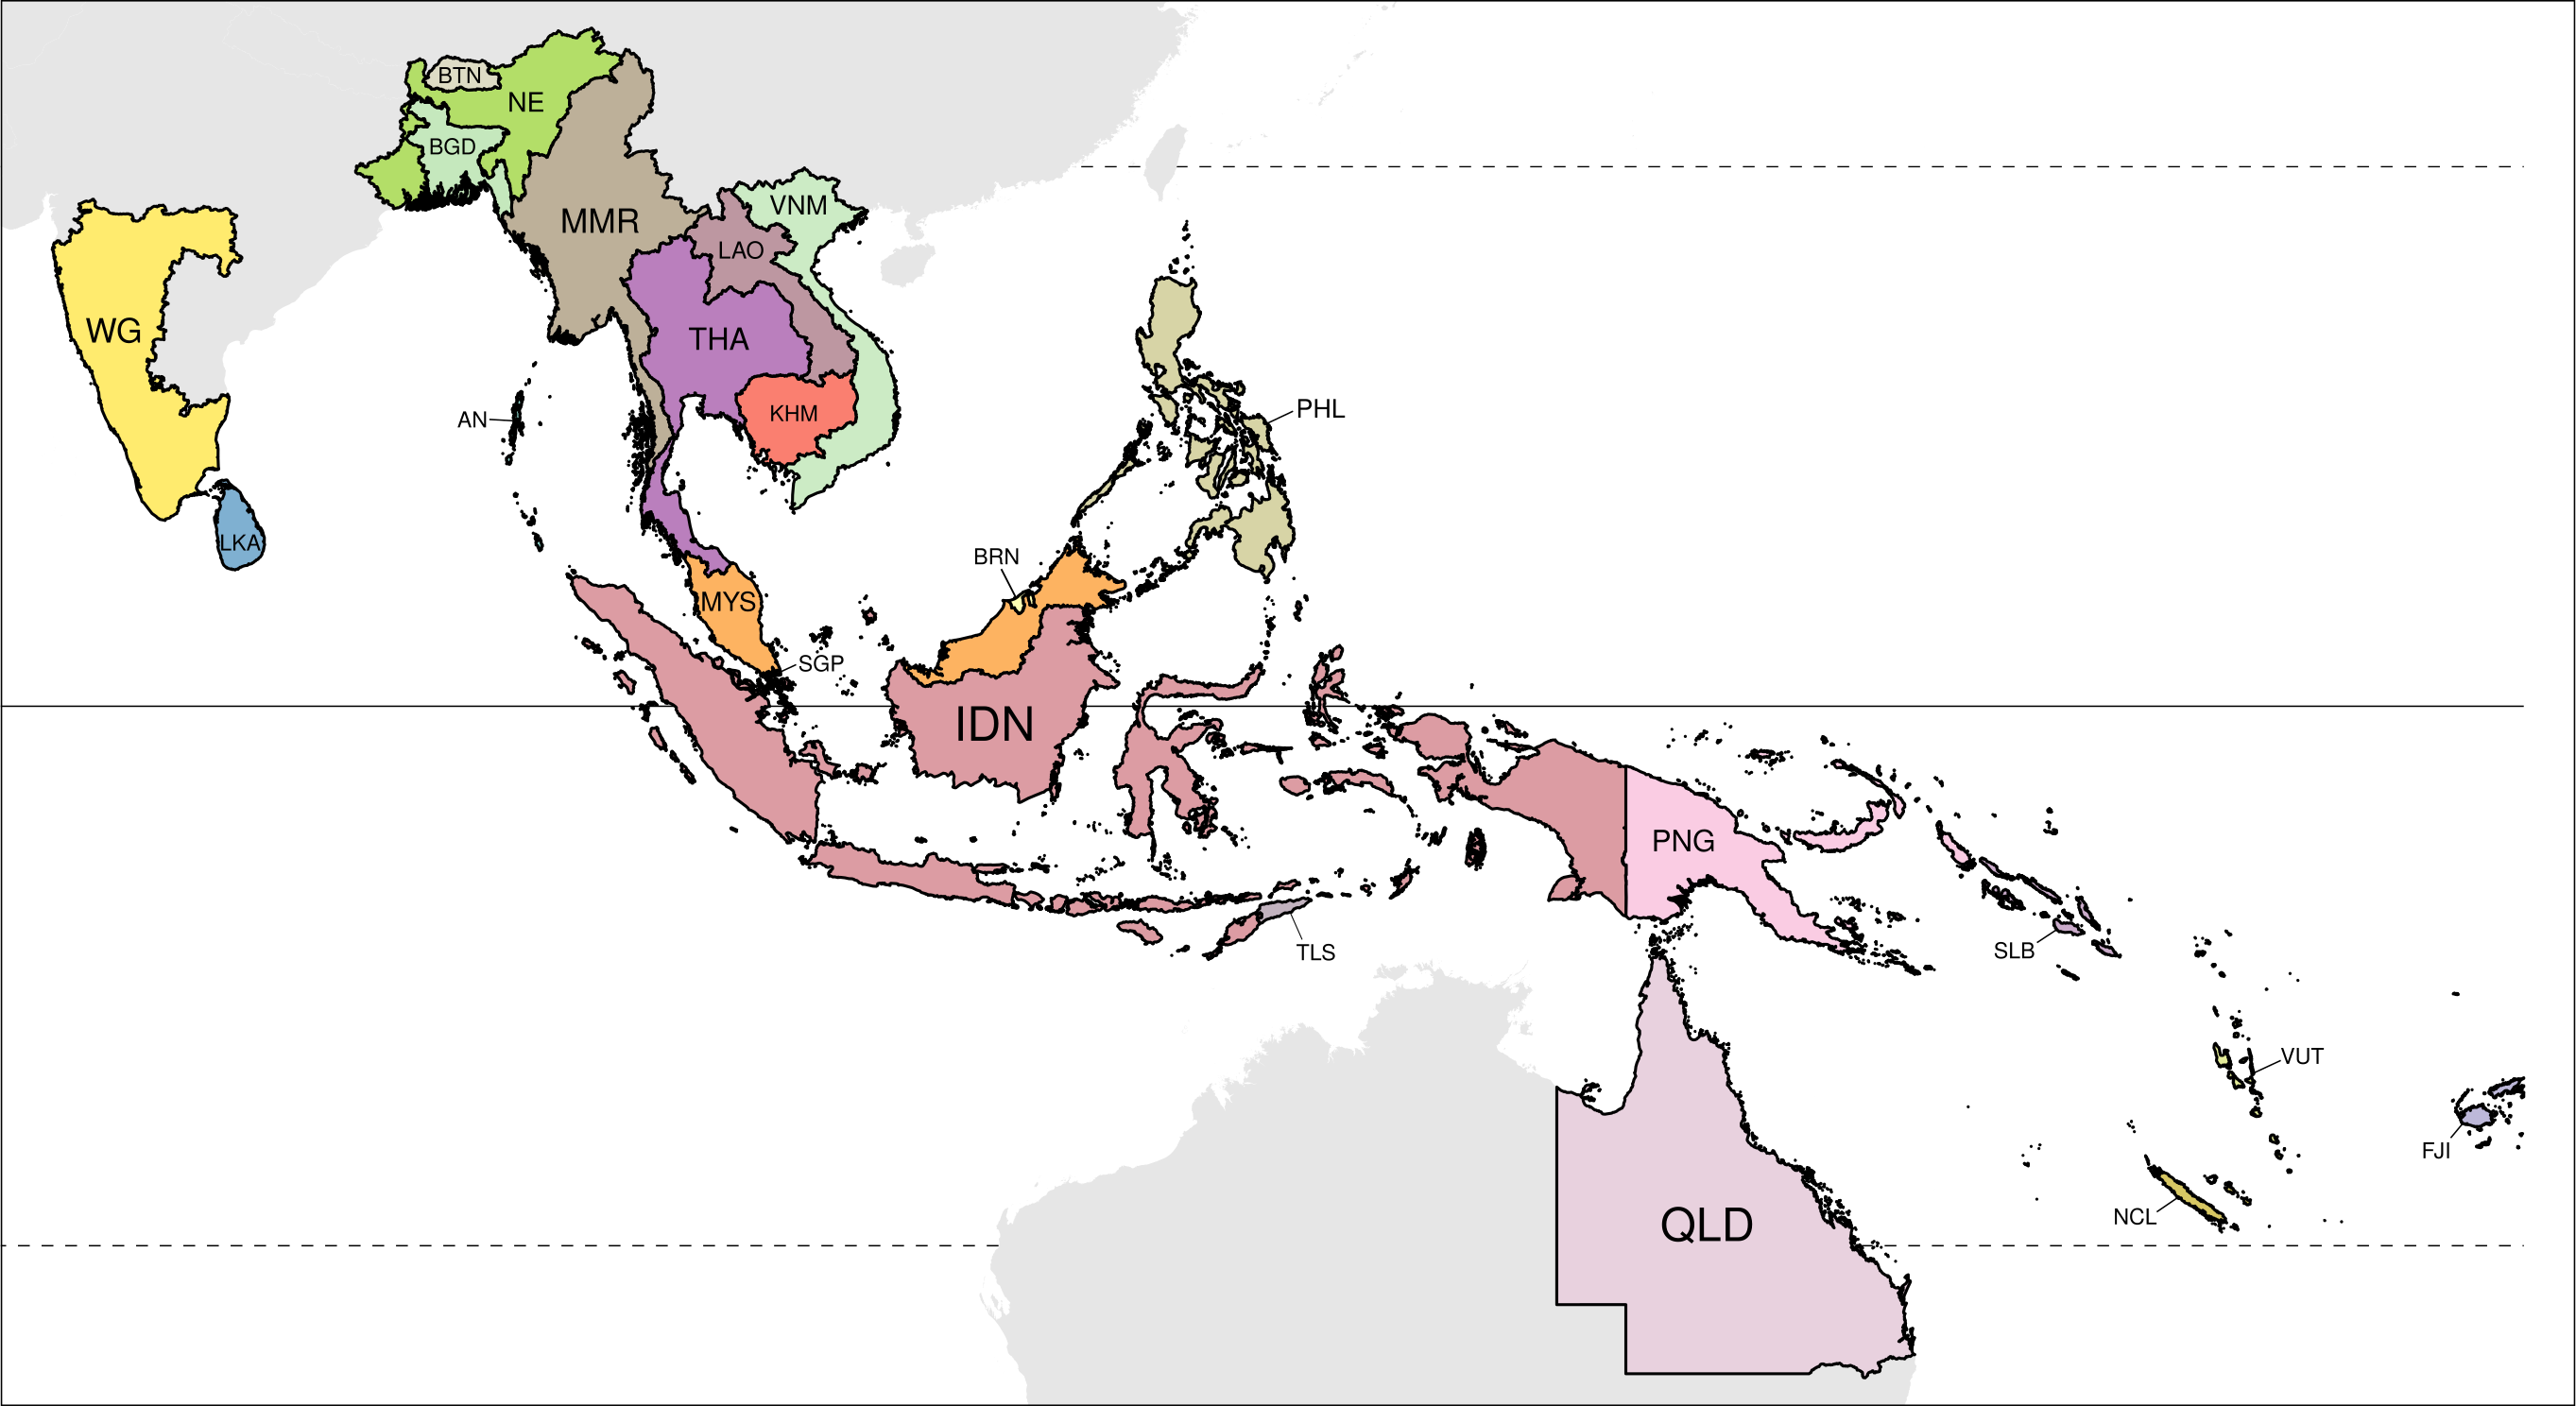
\includegraphics[width=0.32\textwidth]{figs/sm/study_areas_Asia}
\textbf{The 119 study areas in the 3 continents}
\end{center}
\end{frame}

\begin{frame}[label={sec:org3d41cd1}]{Spatial probability of deforestation}
\centering 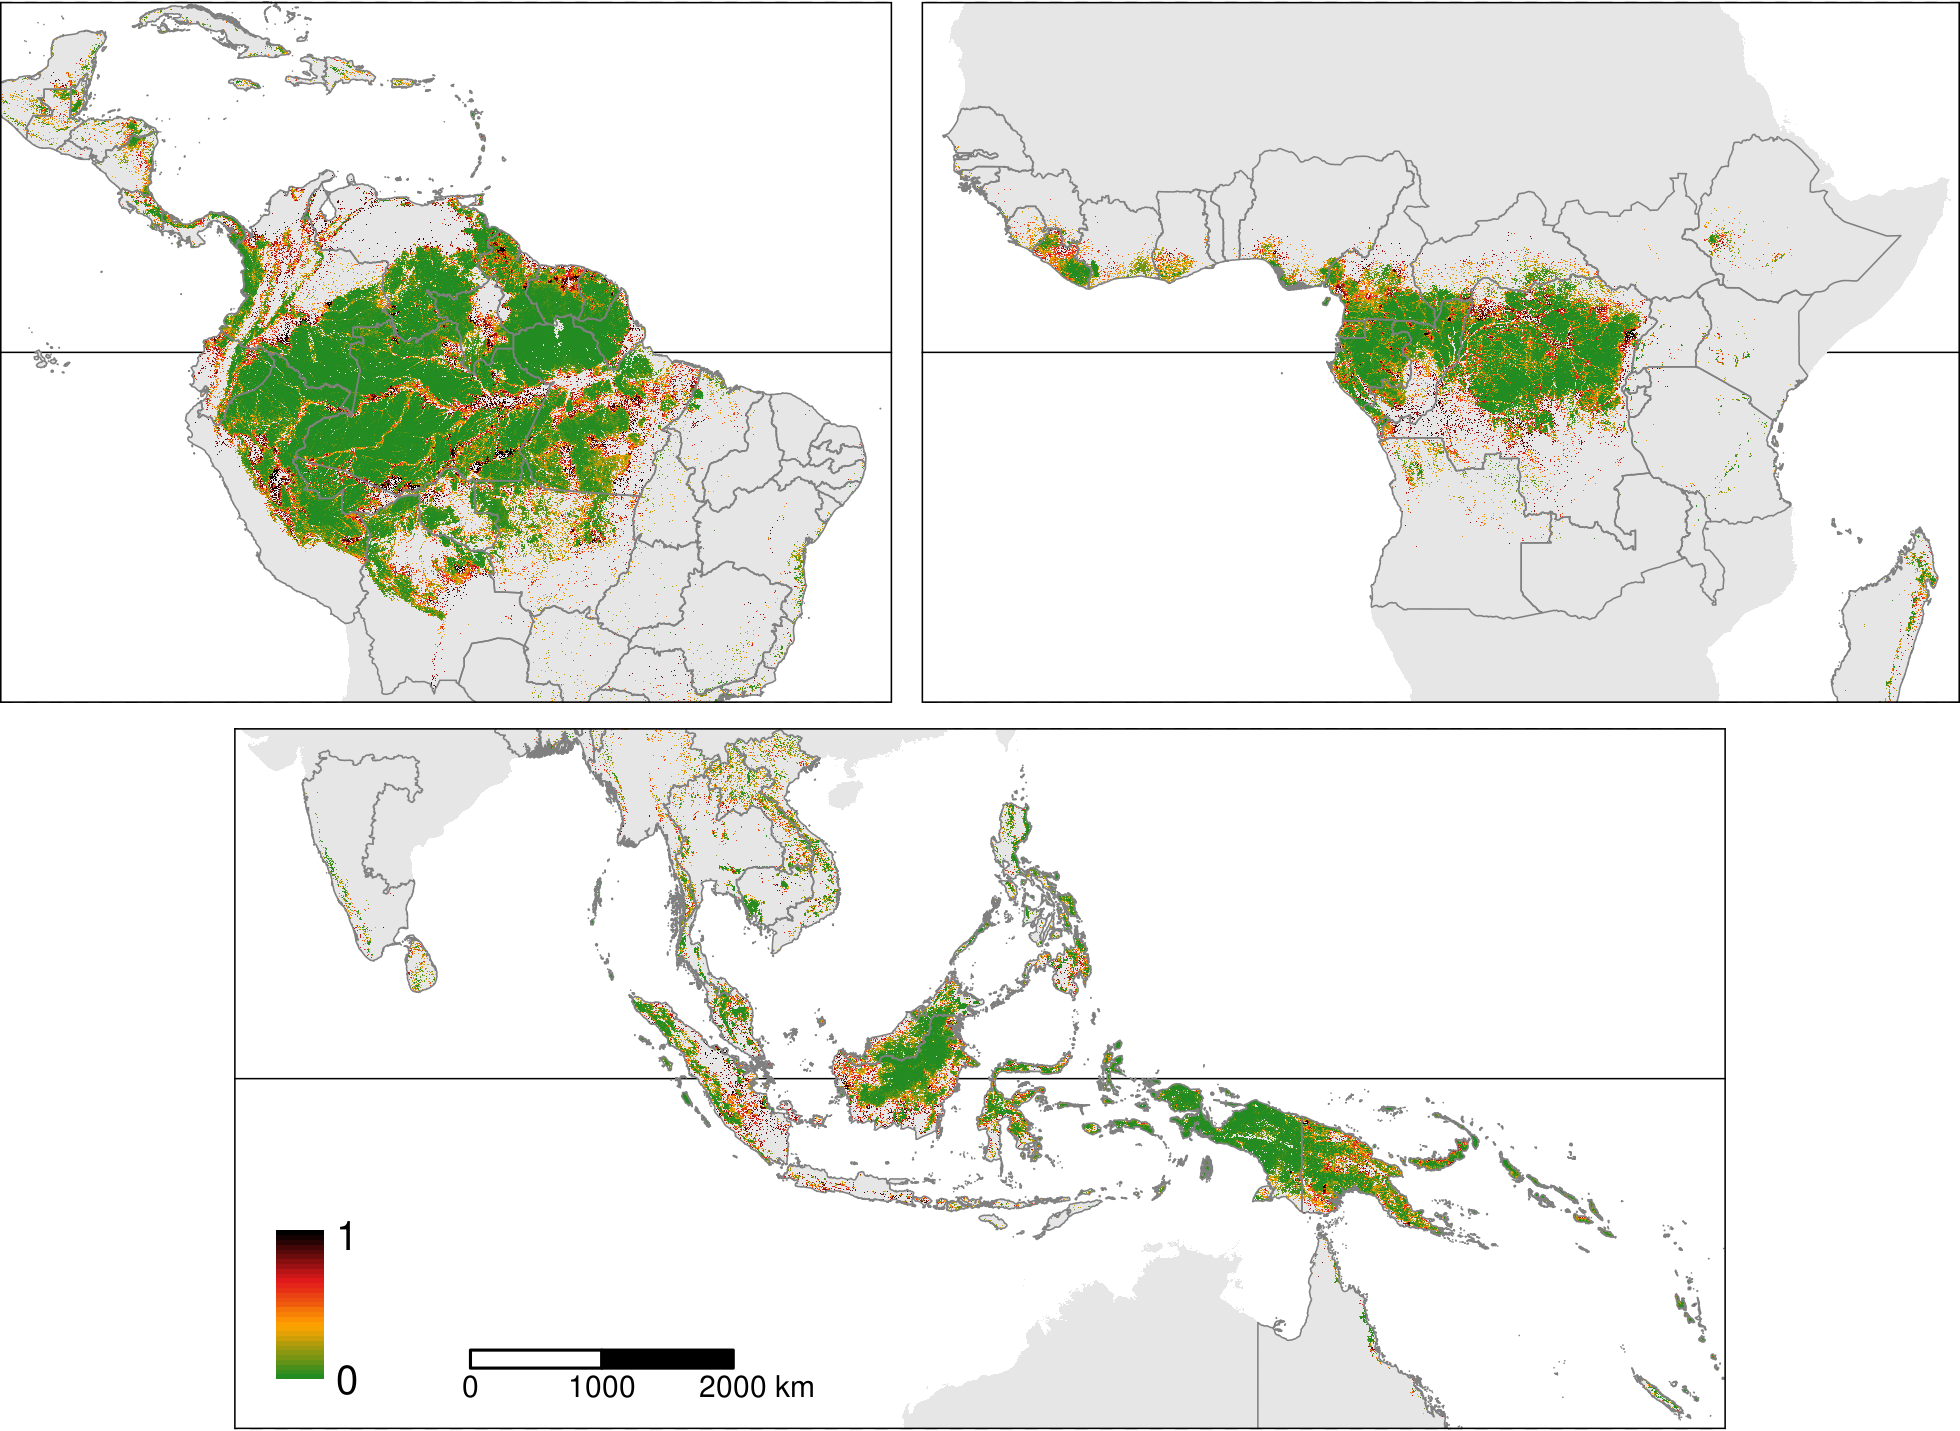
\includegraphics[width=0.7\textwidth]{figs/article/prob}

\structure{Pantropical map of the spatial probability of deforestation}

Article in review: \href{https://doi.org/10.1101/2022.03.22.485306}{10.1101/2022.03.22.485306}

\url{https://forestatrisk.cirad.fr/maps.html}
\end{frame}

\subsection{Other case-studies}
\label{sec:org2349e0d}

\begin{frame}[label={sec:org79f4f75}]{Other case-studies}
\begin{itemize}
\item Impact of mining activities in New-Caledonia.
\item National Parks vs. Community Managed Forests in Madagascar.
\item \(\ldots\)
\end{itemize}
\end{frame}

% %%%%%%%%%%%%%%%%%%%%%%%%%%%%%%%%%%%%%%%%%%%%%%%%%%%%%%%%%%

{
  % Use background image
  \usebackgroundtemplate{%
    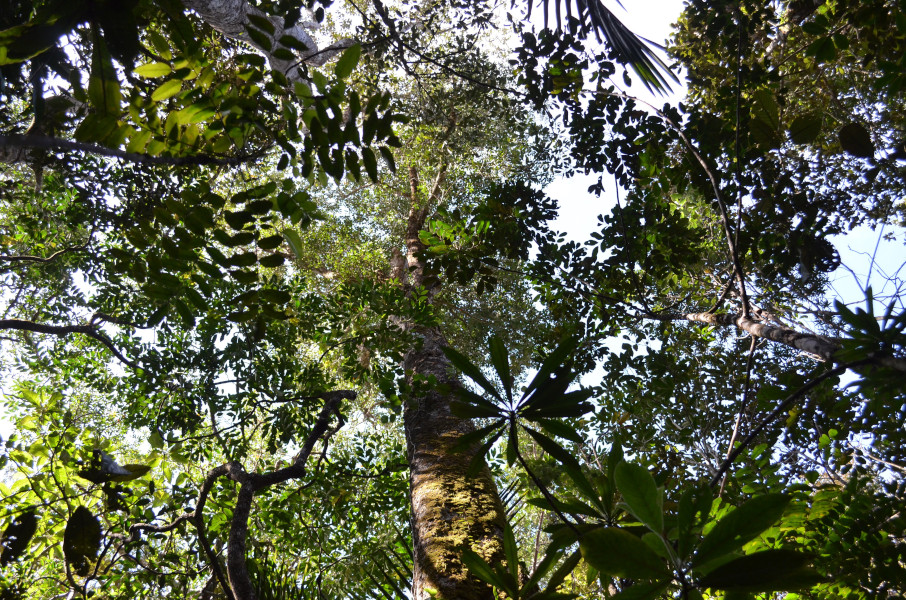
\includegraphics[keepaspectratio=true, height=\paperheight]{figs/Canopy-NC}
  }
  \setbeamertemplate{navigation symbols}{}
  % Remove shadow from block
  \setbeamertemplate{blocks}[rounded][shadow=false]
  \begin{frame}[plain]
  	\vspace*{\stretch{100}} 
    \begin{block}{}
      \begin{center}
        \ldots~Thank you for attention~\ldots \\
        \url{https://forestatrisk.cirad.fr} \\
        
\includegraphics[width=0.8\textwidth]{figs/partners_logos}
      \end{center}
    \end{block}
  \end{frame}
}
\end{document}